
% Default to the notebook output style

    


% Inherit from the specified cell style.




    
\documentclass[11pt]{article}

    
    
    \usepackage[T1]{fontenc}
    % Nicer default font (+ math font) than Computer Modern for most use cases
    \usepackage{mathpazo}

    % Basic figure setup, for now with no caption control since it's done
    % automatically by Pandoc (which extracts ![](path) syntax from Markdown).
    \usepackage{graphicx}
    % We will generate all images so they have a width \maxwidth. This means
    % that they will get their normal width if they fit onto the page, but
    % are scaled down if they would overflow the margins.
    \makeatletter
    \def\maxwidth{\ifdim\Gin@nat@width>\linewidth\linewidth
    \else\Gin@nat@width\fi}
    \makeatother
    \let\Oldincludegraphics\includegraphics
    % Set max figure width to be 80% of text width, for now hardcoded.
    \renewcommand{\includegraphics}[1]{\Oldincludegraphics[width=.8\maxwidth]{#1}}
    % Ensure that by default, figures have no caption (until we provide a
    % proper Figure object with a Caption API and a way to capture that
    % in the conversion process - todo).
    \usepackage{caption}
    \DeclareCaptionLabelFormat{nolabel}{}
    \captionsetup{labelformat=nolabel}

    \usepackage{adjustbox} % Used to constrain images to a maximum size 
    \usepackage{xcolor} % Allow colors to be defined
    \usepackage{enumerate} % Needed for markdown enumerations to work
    \usepackage{geometry} % Used to adjust the document margins
    \usepackage{amsmath} % Equations
    \usepackage{amssymb} % Equations
    \usepackage{textcomp} % defines textquotesingle
    % Hack from http://tex.stackexchange.com/a/47451/13684:
    \AtBeginDocument{%
        \def\PYZsq{\textquotesingle}% Upright quotes in Pygmentized code
    }
    \usepackage{upquote} % Upright quotes for verbatim code
    \usepackage{eurosym} % defines \euro
    \usepackage[mathletters]{ucs} % Extended unicode (utf-8) support
    \usepackage[utf8x]{inputenc} % Allow utf-8 characters in the tex document
    \usepackage{fancyvrb} % verbatim replacement that allows latex
    \usepackage{grffile} % extends the file name processing of package graphics 
                         % to support a larger range 
    % The hyperref package gives us a pdf with properly built
    % internal navigation ('pdf bookmarks' for the table of contents,
    % internal cross-reference links, web links for URLs, etc.)
    \usepackage{hyperref}
    \usepackage{longtable} % longtable support required by pandoc >1.10
    \usepackage{booktabs}  % table support for pandoc > 1.12.2
    \usepackage[inline]{enumitem} % IRkernel/repr support (it uses the enumerate* environment)
    \usepackage[normalem]{ulem} % ulem is needed to support strikethroughs (\sout)
                                % normalem makes italics be italics, not underlines
    

    
    
    % Colors for the hyperref package
    \definecolor{urlcolor}{rgb}{0,.145,.698}
    \definecolor{linkcolor}{rgb}{.71,0.21,0.01}
    \definecolor{citecolor}{rgb}{.12,.54,.11}

    % ANSI colors
    \definecolor{ansi-black}{HTML}{3E424D}
    \definecolor{ansi-black-intense}{HTML}{282C36}
    \definecolor{ansi-red}{HTML}{E75C58}
    \definecolor{ansi-red-intense}{HTML}{B22B31}
    \definecolor{ansi-green}{HTML}{00A250}
    \definecolor{ansi-green-intense}{HTML}{007427}
    \definecolor{ansi-yellow}{HTML}{DDB62B}
    \definecolor{ansi-yellow-intense}{HTML}{B27D12}
    \definecolor{ansi-blue}{HTML}{208FFB}
    \definecolor{ansi-blue-intense}{HTML}{0065CA}
    \definecolor{ansi-magenta}{HTML}{D160C4}
    \definecolor{ansi-magenta-intense}{HTML}{A03196}
    \definecolor{ansi-cyan}{HTML}{60C6C8}
    \definecolor{ansi-cyan-intense}{HTML}{258F8F}
    \definecolor{ansi-white}{HTML}{C5C1B4}
    \definecolor{ansi-white-intense}{HTML}{A1A6B2}

    % commands and environments needed by pandoc snippets
    % extracted from the output of `pandoc -s`
    \providecommand{\tightlist}{%
      \setlength{\itemsep}{0pt}\setlength{\parskip}{0pt}}
    \DefineVerbatimEnvironment{Highlighting}{Verbatim}{commandchars=\\\{\}}
    % Add ',fontsize=\small' for more characters per line
    \newenvironment{Shaded}{}{}
    \newcommand{\KeywordTok}[1]{\textcolor[rgb]{0.00,0.44,0.13}{\textbf{{#1}}}}
    \newcommand{\DataTypeTok}[1]{\textcolor[rgb]{0.56,0.13,0.00}{{#1}}}
    \newcommand{\DecValTok}[1]{\textcolor[rgb]{0.25,0.63,0.44}{{#1}}}
    \newcommand{\BaseNTok}[1]{\textcolor[rgb]{0.25,0.63,0.44}{{#1}}}
    \newcommand{\FloatTok}[1]{\textcolor[rgb]{0.25,0.63,0.44}{{#1}}}
    \newcommand{\CharTok}[1]{\textcolor[rgb]{0.25,0.44,0.63}{{#1}}}
    \newcommand{\StringTok}[1]{\textcolor[rgb]{0.25,0.44,0.63}{{#1}}}
    \newcommand{\CommentTok}[1]{\textcolor[rgb]{0.38,0.63,0.69}{\textit{{#1}}}}
    \newcommand{\OtherTok}[1]{\textcolor[rgb]{0.00,0.44,0.13}{{#1}}}
    \newcommand{\AlertTok}[1]{\textcolor[rgb]{1.00,0.00,0.00}{\textbf{{#1}}}}
    \newcommand{\FunctionTok}[1]{\textcolor[rgb]{0.02,0.16,0.49}{{#1}}}
    \newcommand{\RegionMarkerTok}[1]{{#1}}
    \newcommand{\ErrorTok}[1]{\textcolor[rgb]{1.00,0.00,0.00}{\textbf{{#1}}}}
    \newcommand{\NormalTok}[1]{{#1}}
    
    % Additional commands for more recent versions of Pandoc
    \newcommand{\ConstantTok}[1]{\textcolor[rgb]{0.53,0.00,0.00}{{#1}}}
    \newcommand{\SpecialCharTok}[1]{\textcolor[rgb]{0.25,0.44,0.63}{{#1}}}
    \newcommand{\VerbatimStringTok}[1]{\textcolor[rgb]{0.25,0.44,0.63}{{#1}}}
    \newcommand{\SpecialStringTok}[1]{\textcolor[rgb]{0.73,0.40,0.53}{{#1}}}
    \newcommand{\ImportTok}[1]{{#1}}
    \newcommand{\DocumentationTok}[1]{\textcolor[rgb]{0.73,0.13,0.13}{\textit{{#1}}}}
    \newcommand{\AnnotationTok}[1]{\textcolor[rgb]{0.38,0.63,0.69}{\textbf{\textit{{#1}}}}}
    \newcommand{\CommentVarTok}[1]{\textcolor[rgb]{0.38,0.63,0.69}{\textbf{\textit{{#1}}}}}
    \newcommand{\VariableTok}[1]{\textcolor[rgb]{0.10,0.09,0.49}{{#1}}}
    \newcommand{\ControlFlowTok}[1]{\textcolor[rgb]{0.00,0.44,0.13}{\textbf{{#1}}}}
    \newcommand{\OperatorTok}[1]{\textcolor[rgb]{0.40,0.40,0.40}{{#1}}}
    \newcommand{\BuiltInTok}[1]{{#1}}
    \newcommand{\ExtensionTok}[1]{{#1}}
    \newcommand{\PreprocessorTok}[1]{\textcolor[rgb]{0.74,0.48,0.00}{{#1}}}
    \newcommand{\AttributeTok}[1]{\textcolor[rgb]{0.49,0.56,0.16}{{#1}}}
    \newcommand{\InformationTok}[1]{\textcolor[rgb]{0.38,0.63,0.69}{\textbf{\textit{{#1}}}}}
    \newcommand{\WarningTok}[1]{\textcolor[rgb]{0.38,0.63,0.69}{\textbf{\textit{{#1}}}}}
    
    
    % Define a nice break command that doesn't care if a line doesn't already
    % exist.
    \def\br{\hspace*{\fill} \\* }
    % Math Jax compatability definitions
    \def\gt{>}
    \def\lt{<}
    % Document parameters
    \title{Projecy}
    
    
    

    % Pygments definitions
    
\makeatletter
\def\PY@reset{\let\PY@it=\relax \let\PY@bf=\relax%
    \let\PY@ul=\relax \let\PY@tc=\relax%
    \let\PY@bc=\relax \let\PY@ff=\relax}
\def\PY@tok#1{\csname PY@tok@#1\endcsname}
\def\PY@toks#1+{\ifx\relax#1\empty\else%
    \PY@tok{#1}\expandafter\PY@toks\fi}
\def\PY@do#1{\PY@bc{\PY@tc{\PY@ul{%
    \PY@it{\PY@bf{\PY@ff{#1}}}}}}}
\def\PY#1#2{\PY@reset\PY@toks#1+\relax+\PY@do{#2}}

\expandafter\def\csname PY@tok@w\endcsname{\def\PY@tc##1{\textcolor[rgb]{0.73,0.73,0.73}{##1}}}
\expandafter\def\csname PY@tok@c\endcsname{\let\PY@it=\textit\def\PY@tc##1{\textcolor[rgb]{0.25,0.50,0.50}{##1}}}
\expandafter\def\csname PY@tok@cp\endcsname{\def\PY@tc##1{\textcolor[rgb]{0.74,0.48,0.00}{##1}}}
\expandafter\def\csname PY@tok@k\endcsname{\let\PY@bf=\textbf\def\PY@tc##1{\textcolor[rgb]{0.00,0.50,0.00}{##1}}}
\expandafter\def\csname PY@tok@kp\endcsname{\def\PY@tc##1{\textcolor[rgb]{0.00,0.50,0.00}{##1}}}
\expandafter\def\csname PY@tok@kt\endcsname{\def\PY@tc##1{\textcolor[rgb]{0.69,0.00,0.25}{##1}}}
\expandafter\def\csname PY@tok@o\endcsname{\def\PY@tc##1{\textcolor[rgb]{0.40,0.40,0.40}{##1}}}
\expandafter\def\csname PY@tok@ow\endcsname{\let\PY@bf=\textbf\def\PY@tc##1{\textcolor[rgb]{0.67,0.13,1.00}{##1}}}
\expandafter\def\csname PY@tok@nb\endcsname{\def\PY@tc##1{\textcolor[rgb]{0.00,0.50,0.00}{##1}}}
\expandafter\def\csname PY@tok@nf\endcsname{\def\PY@tc##1{\textcolor[rgb]{0.00,0.00,1.00}{##1}}}
\expandafter\def\csname PY@tok@nc\endcsname{\let\PY@bf=\textbf\def\PY@tc##1{\textcolor[rgb]{0.00,0.00,1.00}{##1}}}
\expandafter\def\csname PY@tok@nn\endcsname{\let\PY@bf=\textbf\def\PY@tc##1{\textcolor[rgb]{0.00,0.00,1.00}{##1}}}
\expandafter\def\csname PY@tok@ne\endcsname{\let\PY@bf=\textbf\def\PY@tc##1{\textcolor[rgb]{0.82,0.25,0.23}{##1}}}
\expandafter\def\csname PY@tok@nv\endcsname{\def\PY@tc##1{\textcolor[rgb]{0.10,0.09,0.49}{##1}}}
\expandafter\def\csname PY@tok@no\endcsname{\def\PY@tc##1{\textcolor[rgb]{0.53,0.00,0.00}{##1}}}
\expandafter\def\csname PY@tok@nl\endcsname{\def\PY@tc##1{\textcolor[rgb]{0.63,0.63,0.00}{##1}}}
\expandafter\def\csname PY@tok@ni\endcsname{\let\PY@bf=\textbf\def\PY@tc##1{\textcolor[rgb]{0.60,0.60,0.60}{##1}}}
\expandafter\def\csname PY@tok@na\endcsname{\def\PY@tc##1{\textcolor[rgb]{0.49,0.56,0.16}{##1}}}
\expandafter\def\csname PY@tok@nt\endcsname{\let\PY@bf=\textbf\def\PY@tc##1{\textcolor[rgb]{0.00,0.50,0.00}{##1}}}
\expandafter\def\csname PY@tok@nd\endcsname{\def\PY@tc##1{\textcolor[rgb]{0.67,0.13,1.00}{##1}}}
\expandafter\def\csname PY@tok@s\endcsname{\def\PY@tc##1{\textcolor[rgb]{0.73,0.13,0.13}{##1}}}
\expandafter\def\csname PY@tok@sd\endcsname{\let\PY@it=\textit\def\PY@tc##1{\textcolor[rgb]{0.73,0.13,0.13}{##1}}}
\expandafter\def\csname PY@tok@si\endcsname{\let\PY@bf=\textbf\def\PY@tc##1{\textcolor[rgb]{0.73,0.40,0.53}{##1}}}
\expandafter\def\csname PY@tok@se\endcsname{\let\PY@bf=\textbf\def\PY@tc##1{\textcolor[rgb]{0.73,0.40,0.13}{##1}}}
\expandafter\def\csname PY@tok@sr\endcsname{\def\PY@tc##1{\textcolor[rgb]{0.73,0.40,0.53}{##1}}}
\expandafter\def\csname PY@tok@ss\endcsname{\def\PY@tc##1{\textcolor[rgb]{0.10,0.09,0.49}{##1}}}
\expandafter\def\csname PY@tok@sx\endcsname{\def\PY@tc##1{\textcolor[rgb]{0.00,0.50,0.00}{##1}}}
\expandafter\def\csname PY@tok@m\endcsname{\def\PY@tc##1{\textcolor[rgb]{0.40,0.40,0.40}{##1}}}
\expandafter\def\csname PY@tok@gh\endcsname{\let\PY@bf=\textbf\def\PY@tc##1{\textcolor[rgb]{0.00,0.00,0.50}{##1}}}
\expandafter\def\csname PY@tok@gu\endcsname{\let\PY@bf=\textbf\def\PY@tc##1{\textcolor[rgb]{0.50,0.00,0.50}{##1}}}
\expandafter\def\csname PY@tok@gd\endcsname{\def\PY@tc##1{\textcolor[rgb]{0.63,0.00,0.00}{##1}}}
\expandafter\def\csname PY@tok@gi\endcsname{\def\PY@tc##1{\textcolor[rgb]{0.00,0.63,0.00}{##1}}}
\expandafter\def\csname PY@tok@gr\endcsname{\def\PY@tc##1{\textcolor[rgb]{1.00,0.00,0.00}{##1}}}
\expandafter\def\csname PY@tok@ge\endcsname{\let\PY@it=\textit}
\expandafter\def\csname PY@tok@gs\endcsname{\let\PY@bf=\textbf}
\expandafter\def\csname PY@tok@gp\endcsname{\let\PY@bf=\textbf\def\PY@tc##1{\textcolor[rgb]{0.00,0.00,0.50}{##1}}}
\expandafter\def\csname PY@tok@go\endcsname{\def\PY@tc##1{\textcolor[rgb]{0.53,0.53,0.53}{##1}}}
\expandafter\def\csname PY@tok@gt\endcsname{\def\PY@tc##1{\textcolor[rgb]{0.00,0.27,0.87}{##1}}}
\expandafter\def\csname PY@tok@err\endcsname{\def\PY@bc##1{\setlength{\fboxsep}{0pt}\fcolorbox[rgb]{1.00,0.00,0.00}{1,1,1}{\strut ##1}}}
\expandafter\def\csname PY@tok@kc\endcsname{\let\PY@bf=\textbf\def\PY@tc##1{\textcolor[rgb]{0.00,0.50,0.00}{##1}}}
\expandafter\def\csname PY@tok@kd\endcsname{\let\PY@bf=\textbf\def\PY@tc##1{\textcolor[rgb]{0.00,0.50,0.00}{##1}}}
\expandafter\def\csname PY@tok@kn\endcsname{\let\PY@bf=\textbf\def\PY@tc##1{\textcolor[rgb]{0.00,0.50,0.00}{##1}}}
\expandafter\def\csname PY@tok@kr\endcsname{\let\PY@bf=\textbf\def\PY@tc##1{\textcolor[rgb]{0.00,0.50,0.00}{##1}}}
\expandafter\def\csname PY@tok@bp\endcsname{\def\PY@tc##1{\textcolor[rgb]{0.00,0.50,0.00}{##1}}}
\expandafter\def\csname PY@tok@fm\endcsname{\def\PY@tc##1{\textcolor[rgb]{0.00,0.00,1.00}{##1}}}
\expandafter\def\csname PY@tok@vc\endcsname{\def\PY@tc##1{\textcolor[rgb]{0.10,0.09,0.49}{##1}}}
\expandafter\def\csname PY@tok@vg\endcsname{\def\PY@tc##1{\textcolor[rgb]{0.10,0.09,0.49}{##1}}}
\expandafter\def\csname PY@tok@vi\endcsname{\def\PY@tc##1{\textcolor[rgb]{0.10,0.09,0.49}{##1}}}
\expandafter\def\csname PY@tok@vm\endcsname{\def\PY@tc##1{\textcolor[rgb]{0.10,0.09,0.49}{##1}}}
\expandafter\def\csname PY@tok@sa\endcsname{\def\PY@tc##1{\textcolor[rgb]{0.73,0.13,0.13}{##1}}}
\expandafter\def\csname PY@tok@sb\endcsname{\def\PY@tc##1{\textcolor[rgb]{0.73,0.13,0.13}{##1}}}
\expandafter\def\csname PY@tok@sc\endcsname{\def\PY@tc##1{\textcolor[rgb]{0.73,0.13,0.13}{##1}}}
\expandafter\def\csname PY@tok@dl\endcsname{\def\PY@tc##1{\textcolor[rgb]{0.73,0.13,0.13}{##1}}}
\expandafter\def\csname PY@tok@s2\endcsname{\def\PY@tc##1{\textcolor[rgb]{0.73,0.13,0.13}{##1}}}
\expandafter\def\csname PY@tok@sh\endcsname{\def\PY@tc##1{\textcolor[rgb]{0.73,0.13,0.13}{##1}}}
\expandafter\def\csname PY@tok@s1\endcsname{\def\PY@tc##1{\textcolor[rgb]{0.73,0.13,0.13}{##1}}}
\expandafter\def\csname PY@tok@mb\endcsname{\def\PY@tc##1{\textcolor[rgb]{0.40,0.40,0.40}{##1}}}
\expandafter\def\csname PY@tok@mf\endcsname{\def\PY@tc##1{\textcolor[rgb]{0.40,0.40,0.40}{##1}}}
\expandafter\def\csname PY@tok@mh\endcsname{\def\PY@tc##1{\textcolor[rgb]{0.40,0.40,0.40}{##1}}}
\expandafter\def\csname PY@tok@mi\endcsname{\def\PY@tc##1{\textcolor[rgb]{0.40,0.40,0.40}{##1}}}
\expandafter\def\csname PY@tok@il\endcsname{\def\PY@tc##1{\textcolor[rgb]{0.40,0.40,0.40}{##1}}}
\expandafter\def\csname PY@tok@mo\endcsname{\def\PY@tc##1{\textcolor[rgb]{0.40,0.40,0.40}{##1}}}
\expandafter\def\csname PY@tok@ch\endcsname{\let\PY@it=\textit\def\PY@tc##1{\textcolor[rgb]{0.25,0.50,0.50}{##1}}}
\expandafter\def\csname PY@tok@cm\endcsname{\let\PY@it=\textit\def\PY@tc##1{\textcolor[rgb]{0.25,0.50,0.50}{##1}}}
\expandafter\def\csname PY@tok@cpf\endcsname{\let\PY@it=\textit\def\PY@tc##1{\textcolor[rgb]{0.25,0.50,0.50}{##1}}}
\expandafter\def\csname PY@tok@c1\endcsname{\let\PY@it=\textit\def\PY@tc##1{\textcolor[rgb]{0.25,0.50,0.50}{##1}}}
\expandafter\def\csname PY@tok@cs\endcsname{\let\PY@it=\textit\def\PY@tc##1{\textcolor[rgb]{0.25,0.50,0.50}{##1}}}

\def\PYZbs{\char`\\}
\def\PYZus{\char`\_}
\def\PYZob{\char`\{}
\def\PYZcb{\char`\}}
\def\PYZca{\char`\^}
\def\PYZam{\char`\&}
\def\PYZlt{\char`\<}
\def\PYZgt{\char`\>}
\def\PYZsh{\char`\#}
\def\PYZpc{\char`\%}
\def\PYZdl{\char`\$}
\def\PYZhy{\char`\-}
\def\PYZsq{\char`\'}
\def\PYZdq{\char`\"}
\def\PYZti{\char`\~}
% for compatibility with earlier versions
\def\PYZat{@}
\def\PYZlb{[}
\def\PYZrb{]}
\makeatother


    % Exact colors from NB
    \definecolor{incolor}{rgb}{0.0, 0.0, 0.5}
    \definecolor{outcolor}{rgb}{0.545, 0.0, 0.0}



    
    % Prevent overflowing lines due to hard-to-break entities
    \sloppy 
    % Setup hyperref package
    \hypersetup{
      breaklinks=true,  % so long urls are correctly broken across lines
      colorlinks=true,
      urlcolor=urlcolor,
      linkcolor=linkcolor,
      citecolor=citecolor,
      }
    % Slightly bigger margins than the latex defaults
    
    \geometry{verbose,tmargin=1in,bmargin=1in,lmargin=1in,rmargin=1in}
    
    

    \begin{document}
    
    
    \maketitle
    
    

    
    \subsubsection{Environment initialize}\label{environment-initialize}

    \begin{Verbatim}[commandchars=\\\{\}]
{\color{incolor}In [{\color{incolor}1}]:} \PY{k+kn}{from} \PY{n+nn}{random} \PY{k}{import} \PY{o}{*}
        \PY{k+kn}{import} \PY{n+nn}{numpy} \PY{k}{as} \PY{n+nn}{np}
        \PY{k+kn}{import} \PY{n+nn}{matplotlib}\PY{n+nn}{.}\PY{n+nn}{pyplot} \PY{k}{as} \PY{n+nn}{plt}
\end{Verbatim}


    \begin{Verbatim}[commandchars=\\\{\}]
{\color{incolor}In [{\color{incolor}8}]:} \PY{n}{theta}\PY{o}{=}\PY{p}{[}\PY{o}{.}\PY{l+m+mi}{8}\PY{p}{,}\PY{o}{.}\PY{l+m+mi}{6}\PY{p}{,}\PY{o}{.}\PY{l+m+mi}{5}\PY{p}{]}
        \PY{k}{def} \PY{n+nf}{reward}\PY{p}{(}\PY{n}{arm}\PY{p}{)}\PY{p}{:}
            \PY{n}{seed} \PY{o}{=} \PY{n}{random}\PY{p}{(}\PY{p}{)}
            \PY{k}{if}\PY{p}{(}\PY{n}{seed}\PY{o}{\PYZlt{}}\PY{o}{=}\PY{n}{theta}\PY{p}{[}\PY{n}{arm}\PY{p}{]}\PY{p}{)}\PY{p}{:}
                \PY{k}{return} \PY{l+m+mi}{1}
            \PY{k}{return} \PY{l+m+mi}{0}
\end{Verbatim}


    ============================================================================================================

    \section{Content}\label{content}

\begin{itemize}
\item
  Algorithm code
\item
  Section \ref{ceb5e28892greedy-algorithm}
\item
  Section \ref{ucb-upper-confidence-bound-algorithm}
\item
  Section \ref{thompson-sampling-ts-algorithm}
\item
  Simulation
\item
  Section \ref{step-0----basic-test}
\item
  Section \ref{step-1----oracle-value}
\item
  Section \ref{step-23----implement-classical-bandit-algorithms-and-run-each-for-200-times}
\item
  Section \ref{step-4----compute-gap-and-compare-algorithms}
\item
  Section \ref{step-5----give-your-understanding-of-the-exploration-exploitation-trade-off-in-bandit-algorithms}
\item
  Section \ref{step-6----dependent-arm}
\item
  Section \ref{step-7----constrained-bandit-learning-problem}
\item
  Section \ref{reference}
\item
  Section \ref{step-e2889e----addition}
\item
  Section \ref{adifferent-algorithms-of-cs-view-procon-improvement}
\end{itemize}

​

    ============================================================================================================

    \section{ε−greedy Algorithm}\label{ux3b5greedy-algorithm}

    \begin{Verbatim}[commandchars=\\\{\}]
{\color{incolor}In [{\color{incolor}12}]:} \PY{k}{class} \PY{n+nc}{Greedy}\PY{p}{:}
             \PY{k}{def} \PY{n+nf}{\PYZus{}\PYZus{}init\PYZus{}\PYZus{}}\PY{p}{(}\PY{n+nb+bp}{self}\PY{p}{,}\PY{n}{v}\PY{p}{)}\PY{p}{:}
                 \PY{n+nb+bp}{self}\PY{o}{.}\PY{n}{counts} \PY{o}{=} \PY{n}{np}\PY{o}{.}\PY{n}{array}\PY{p}{(}\PY{p}{[}\PY{l+m+mi}{0}\PY{p}{,} \PY{l+m+mi}{0}\PY{p}{,} \PY{l+m+mi}{0}\PY{p}{]}\PY{p}{)}
                 \PY{n+nb+bp}{self}\PY{o}{.}\PY{n}{nearTheta} \PY{o}{=} \PY{n}{np}\PY{o}{.}\PY{n}{array}\PY{p}{(}\PY{p}{[}\PY{l+m+mi}{0}\PY{p}{,} \PY{l+m+mi}{0}\PY{p}{,} \PY{l+m+mi}{0}\PY{p}{]}\PY{p}{,} \PY{n}{dtype}\PY{o}{=}\PY{n}{np}\PY{o}{.}\PY{n}{float16}\PY{p}{)}
                 \PY{n+nb+bp}{self}\PY{o}{.}\PY{n}{choicesHistory} \PY{o}{=} \PY{p}{[}\PY{p}{]}
                 \PY{n+nb+bp}{self}\PY{o}{.}\PY{n}{moneyHistory}\PY{o}{=}\PY{p}{[}\PY{p}{]}
                 \PY{n+nb+bp}{self}\PY{o}{.}\PY{n}{variation} \PY{o}{=} \PY{n}{v} \PY{c+c1}{\PYZsh{}突变因子(ε)}
         
             \PY{k}{def} \PY{n+nf}{decide}\PY{p}{(}\PY{n+nb+bp}{self}\PY{p}{)}\PY{p}{:}
                 \PY{n}{seed} \PY{o}{=} \PY{n}{random}\PY{p}{(}\PY{p}{)}
                 \PY{k}{if} \PY{p}{(}\PY{n}{seed} \PY{o}{\PYZlt{}}\PY{o}{=} \PY{n+nb+bp}{self}\PY{o}{.}\PY{n}{variation}\PY{p}{)}\PY{p}{:}
                     \PY{n}{choice} \PY{o}{=} \PY{n}{randint}\PY{p}{(}\PY{l+m+mi}{0}\PY{p}{,} \PY{l+m+mi}{2}\PY{p}{)}
                 \PY{k}{else}\PY{p}{:}
                     \PY{n}{choice}\PY{o}{=}\PY{n+nb+bp}{self}\PY{o}{.}\PY{n}{nearTheta}\PY{o}{.}\PY{n}{argmax}\PY{p}{(}\PY{p}{)}
                 \PY{n}{rewardmoney}\PY{o}{=}\PY{n}{reward}\PY{p}{(}\PY{n}{choice}\PY{p}{)}
                 \PY{n+nb+bp}{self}\PY{o}{.}\PY{n}{choicesHistory}\PY{o}{.}\PY{n}{append}\PY{p}{(}\PY{n}{choice}\PY{p}{)}
                 \PY{n+nb+bp}{self}\PY{o}{.}\PY{n}{counts}\PY{p}{[}\PY{n}{choice}\PY{p}{]}\PY{o}{+}\PY{o}{=}\PY{l+m+mi}{1}
                 \PY{n+nb+bp}{self}\PY{o}{.}\PY{n}{nearTheta}\PY{p}{[}\PY{n}{choice}\PY{p}{]}\PY{o}{+}\PY{o}{=}\PY{p}{(}\PY{n}{rewardmoney}\PY{o}{\PYZhy{}}\PY{n+nb+bp}{self}\PY{o}{.}\PY{n}{nearTheta}\PY{p}{[}\PY{n}{choice}\PY{p}{]}\PY{p}{)}\PY{o}{/}\PY{n+nb+bp}{self}\PY{o}{.}\PY{n}{counts}\PY{p}{[}\PY{n}{choice}\PY{p}{]}
                 \PY{k}{return} \PY{n}{rewardmoney}
             \PY{k}{def} \PY{n+nf}{do}\PY{p}{(}\PY{n+nb+bp}{self}\PY{p}{,}\PY{n}{N}\PY{p}{,}\PY{n}{printresult}\PY{o}{=}\PY{k+kc}{True}\PY{p}{)}\PY{p}{:}
                 \PY{n+nb+bp}{self}\PY{o}{.}\PY{n}{money} \PY{o}{=} \PY{l+m+mi}{0}
                 \PY{n+nb+bp}{self}\PY{o}{.}\PY{n}{trytime} \PY{o}{=} \PY{n}{N}
                 \PY{k}{for} \PY{n}{i} \PY{o+ow}{in} \PY{n+nb}{range}\PY{p}{(}\PY{n}{N}\PY{p}{)}\PY{p}{:}
                     \PY{n+nb+bp}{self}\PY{o}{.}\PY{n}{money} \PY{o}{+}\PY{o}{=} \PY{n+nb+bp}{self}\PY{o}{.}\PY{n}{decide}\PY{p}{(}\PY{p}{)}
                     \PY{n+nb+bp}{self}\PY{o}{.}\PY{n}{moneyHistory}\PY{o}{.}\PY{n}{append}\PY{p}{(}\PY{n+nb+bp}{self}\PY{o}{.}\PY{n}{money}\PY{p}{)}
                 \PY{k}{if} \PY{n}{printresult}\PY{p}{:}
                     \PY{n+nb}{print}\PY{p}{(}\PY{n}{f}\PY{l+s+s2}{\PYZdq{}}\PY{l+s+s2}{Greedy}\PY{l+s+se}{\PYZbs{}n}\PY{l+s+s2}{Money:}\PY{l+s+si}{\PYZob{}self.money\PYZcb{}}\PY{l+s+s2}{ Try:}\PY{l+s+si}{\PYZob{}self.trytime\PYZcb{}}\PY{l+s+s2}{ ratio:}\PY{l+s+s2}{\PYZob{}}\PY{l+s+s2}{self.money / self.trytime\PYZcb{}}\PY{l+s+s2}{\PYZdq{}}\PY{p}{)}
                 \PY{k}{return} \PY{n+nb+bp}{self}\PY{o}{.}\PY{n}{money}
\end{Verbatim}


    \section{UCB (Upper Confidence Bound)
Algorithm}\label{ucb-upper-confidence-bound-algorithm}

    \begin{Verbatim}[commandchars=\\\{\}]
{\color{incolor}In [{\color{incolor}13}]:} \PY{k}{class} \PY{n+nc}{UCB}\PY{p}{:}
             \PY{k}{def} \PY{n+nf}{\PYZus{}\PYZus{}init\PYZus{}\PYZus{}}\PY{p}{(}\PY{n+nb+bp}{self}\PY{p}{,}\PY{n}{c}\PY{o}{=}\PY{l+m+mi}{1}\PY{p}{)}\PY{p}{:}
                 \PY{n+nb+bp}{self}\PY{o}{.}\PY{n}{counts} \PY{o}{=} \PY{n}{np}\PY{o}{.}\PY{n}{array}\PY{p}{(}\PY{p}{[}\PY{l+m+mi}{1}\PY{p}{,} \PY{l+m+mi}{1}\PY{p}{,} \PY{l+m+mi}{1}\PY{p}{]}\PY{p}{)}
                 \PY{n+nb+bp}{self}\PY{o}{.}\PY{n}{neartheta} \PY{o}{=} \PY{n}{np}\PY{o}{.}\PY{n}{array}\PY{p}{(}\PY{p}{[}\PY{n}{reward}\PY{p}{(}\PY{n}{i}\PY{p}{)} \PY{k}{for} \PY{n}{i} \PY{o+ow}{in} \PY{n+nb}{range}\PY{p}{(}\PY{l+m+mi}{3}\PY{p}{)}\PY{p}{]}\PY{p}{,} \PY{n}{dtype}\PY{o}{=}\PY{n}{np}\PY{o}{.}\PY{n}{float16}\PY{p}{)}
                 \PY{n+nb+bp}{self}\PY{o}{.}\PY{n}{constant} \PY{o}{=} \PY{n}{c}
                 \PY{n+nb+bp}{self}\PY{o}{.}\PY{n}{choicesHistory} \PY{o}{=} \PY{p}{[}\PY{l+m+mi}{0}\PY{p}{,} \PY{l+m+mi}{1}\PY{p}{,} \PY{l+m+mi}{2}\PY{p}{]}
                 \PY{n+nb+bp}{self}\PY{o}{.}\PY{n}{moneyHistory}\PY{o}{=}\PY{p}{[}\PY{l+m+mi}{0}\PY{p}{,}\PY{l+m+mi}{0}\PY{p}{,}\PY{l+m+mi}{0}\PY{p}{]}
                 \PY{n+nb+bp}{self}\PY{o}{.}\PY{n}{t}\PY{o}{=}\PY{l+m+mi}{3}
         
         
             \PY{k}{def} \PY{n+nf}{decide}\PY{p}{(}\PY{n+nb+bp}{self}\PY{p}{)}\PY{p}{:}
                 \PY{n+nb+bp}{self}\PY{o}{.}\PY{n}{t}\PY{o}{+}\PY{o}{=}\PY{l+m+mi}{1}
                 \PY{n}{choice}\PY{o}{=}\PY{n}{np}\PY{o}{.}\PY{n}{array}\PY{p}{(}\PY{n+nb+bp}{self}\PY{o}{.}\PY{n}{neartheta}\PY{o}{+}\PY{n+nb+bp}{self}\PY{o}{.}\PY{n}{constant}\PY{o}{*}\PY{n}{np}\PY{o}{.}\PY{n}{sqrt}\PY{p}{(}\PY{l+m+mf}{2.0}\PY{o}{*}\PY{n}{np}\PY{o}{.}\PY{n}{log}\PY{p}{(}\PY{n+nb+bp}{self}\PY{o}{.}\PY{n}{t}\PY{p}{)}\PY{o}{/}\PY{n+nb+bp}{self}\PY{o}{.}\PY{n}{counts}\PY{p}{)}\PY{p}{)}\PY{o}{.}\PY{n}{argmax}\PY{p}{(}\PY{p}{)}
                 \PY{n+nb+bp}{self}\PY{o}{.}\PY{n}{choicesHistory}\PY{o}{.}\PY{n}{append}\PY{p}{(}\PY{n}{choice}\PY{p}{)}
                 \PY{n+nb+bp}{self}\PY{o}{.}\PY{n}{counts}\PY{p}{[}\PY{n}{choice}\PY{p}{]}\PY{o}{+}\PY{o}{=}\PY{l+m+mi}{1}
                 \PY{n}{moneyget}\PY{o}{=}\PY{n}{reward}\PY{p}{(}\PY{n}{choice}\PY{p}{)}
                 \PY{n+nb+bp}{self}\PY{o}{.}\PY{n}{neartheta}\PY{p}{[}\PY{n}{choice}\PY{p}{]}\PY{o}{+}\PY{o}{=}\PY{p}{(}\PY{n}{moneyget}\PY{o}{\PYZhy{}}\PY{n+nb+bp}{self}\PY{o}{.}\PY{n}{neartheta}\PY{p}{[}\PY{n}{choice}\PY{p}{]}\PY{p}{)}\PY{o}{*}\PY{l+m+mf}{1.0}\PY{o}{/}\PY{n+nb+bp}{self}\PY{o}{.}\PY{n}{counts}\PY{p}{[}\PY{n}{choice}\PY{p}{]}
                 \PY{k}{return} \PY{n}{moneyget}
             \PY{k}{def} \PY{n+nf}{do}\PY{p}{(}\PY{n+nb+bp}{self}\PY{p}{,}\PY{n}{N}\PY{p}{,}\PY{n}{printresult}\PY{o}{=}\PY{k+kc}{True}\PY{p}{)}\PY{p}{:}
                 \PY{n+nb+bp}{self}\PY{o}{.}\PY{n}{money} \PY{o}{=} \PY{l+m+mi}{0}
                 \PY{n+nb+bp}{self}\PY{o}{.}\PY{n}{trytime} \PY{o}{=} \PY{n}{N}
                 \PY{n+nb+bp}{self}\PY{o}{.}\PY{n}{money} \PY{o}{+}\PY{o}{=} \PY{n+nb}{sum}\PY{p}{(}\PY{n+nb+bp}{self}\PY{o}{.}\PY{n}{neartheta}\PY{p}{)}
         
                 \PY{k}{for} \PY{n}{i} \PY{o+ow}{in} \PY{n+nb}{range}\PY{p}{(}\PY{n}{N} \PY{o}{\PYZhy{}} \PY{l+m+mi}{3}\PY{p}{)}\PY{p}{:}
                     \PY{n+nb+bp}{self}\PY{o}{.}\PY{n}{money} \PY{o}{+}\PY{o}{=} \PY{n+nb+bp}{self}\PY{o}{.}\PY{n}{decide}\PY{p}{(}\PY{p}{)}
                     \PY{n+nb+bp}{self}\PY{o}{.}\PY{n}{moneyHistory}\PY{o}{.}\PY{n}{append}\PY{p}{(}\PY{n+nb+bp}{self}\PY{o}{.}\PY{n}{money}\PY{p}{)}
                 \PY{k}{if} \PY{n}{printresult}\PY{p}{:}
                     \PY{n+nb}{print}\PY{p}{(}\PY{n}{f}\PY{l+s+s2}{\PYZdq{}}\PY{l+s+s2}{UCB}\PY{l+s+se}{\PYZbs{}n}\PY{l+s+s2}{ Money:}\PY{l+s+si}{\PYZob{}self.money\PYZcb{}}\PY{l+s+s2}{ Try:}\PY{l+s+si}{\PYZob{}self.trytime\PYZcb{}}\PY{l+s+s2}{ ratio:}\PY{l+s+s2}{\PYZob{}}\PY{l+s+s2}{self.money / self.trytime\PYZcb{}}\PY{l+s+s2}{\PYZdq{}}\PY{p}{)}
                 \PY{k}{return} \PY{n+nb+bp}{self}\PY{o}{.}\PY{n}{money}
\end{Verbatim}


    \section{Thompson sampling (TS)
Algorithm}\label{thompson-sampling-ts-algorithm}

    \begin{Verbatim}[commandchars=\\\{\}]
{\color{incolor}In [{\color{incolor}40}]:} \PY{k}{class} \PY{n+nc}{Thompson}\PY{p}{:}
             \PY{k}{def} \PY{n+nf}{\PYZus{}\PYZus{}init\PYZus{}\PYZus{}}\PY{p}{(}\PY{n+nb+bp}{self}\PY{p}{,}\PY{n}{alpha}\PY{o}{=}\PY{l+m+mi}{1}\PY{p}{,}\PY{n}{beta}\PY{o}{=}\PY{l+m+mi}{2}\PY{p}{)}\PY{p}{:}
                 \PY{n+nb+bp}{self}\PY{o}{.}\PY{n}{priorAlpha}\PY{o}{=}\PY{n}{alpha}
                 \PY{n+nb+bp}{self}\PY{o}{.}\PY{n}{priorBeta}\PY{o}{=}\PY{n}{beta}
                 \PY{n+nb+bp}{self}\PY{o}{.}\PY{n}{alpha}\PY{o}{=}\PY{n}{alpha}\PY{o}{*}\PY{n}{np}\PY{o}{.}\PY{n}{array}\PY{p}{(}\PY{p}{[}\PY{l+m+mi}{1}\PY{p}{,}\PY{l+m+mi}{1}\PY{p}{,}\PY{l+m+mi}{1}\PY{p}{]}\PY{p}{)}
                 \PY{n+nb+bp}{self}\PY{o}{.}\PY{n}{beta}\PY{o}{=}\PY{n}{beta}\PY{o}{*}\PY{n}{np}\PY{o}{.}\PY{n}{array}\PY{p}{(}\PY{p}{[}\PY{l+m+mi}{1}\PY{p}{,}\PY{l+m+mi}{1}\PY{p}{,}\PY{l+m+mi}{1}\PY{p}{]}\PY{p}{)}
                 \PY{n+nb+bp}{self}\PY{o}{.}\PY{n}{neartheta} \PY{o}{=} \PY{n}{np}\PY{o}{.}\PY{n}{array}\PY{p}{(}\PY{p}{[}\PY{p}{]}\PY{p}{)}
                 \PY{n+nb+bp}{self}\PY{o}{.}\PY{n}{choicesHistory} \PY{o}{=} \PY{p}{[}\PY{p}{]}
                 \PY{n+nb+bp}{self}\PY{o}{.}\PY{n}{moneyHistory}\PY{o}{=}\PY{p}{[}\PY{p}{]}
         
             \PY{k}{def} \PY{n+nf}{decide}\PY{p}{(}\PY{n+nb+bp}{self}\PY{p}{)}\PY{p}{:}
                 \PY{n}{neartheta} \PY{o}{=} \PY{n}{np}\PY{o}{.}\PY{n}{array}\PY{p}{(}\PY{n}{np}\PY{o}{.}\PY{n}{random}\PY{o}{.}\PY{n}{beta}\PY{p}{(}\PY{n+nb+bp}{self}\PY{o}{.}\PY{n}{alpha}\PY{p}{,} \PY{n+nb+bp}{self}\PY{o}{.}\PY{n}{beta}\PY{p}{)}\PY{p}{)}
                 \PY{n}{choice}\PY{o}{=}\PY{n}{neartheta}\PY{o}{.}\PY{n}{argmax}\PY{p}{(}\PY{p}{)}
                 \PY{n+nb+bp}{self}\PY{o}{.}\PY{n}{choicesHistory}\PY{o}{.}\PY{n}{append}\PY{p}{(}\PY{n}{choice}\PY{p}{)}
                 \PY{n}{moneyget}\PY{o}{=}\PY{n}{reward}\PY{p}{(}\PY{n}{choice}\PY{p}{)}
                 \PY{n+nb+bp}{self}\PY{o}{.}\PY{n}{alpha}\PY{p}{[}\PY{n}{choice}\PY{p}{]}\PY{o}{+}\PY{o}{=}\PY{n}{moneyget}
                 \PY{n+nb+bp}{self}\PY{o}{.}\PY{n}{beta}\PY{p}{[}\PY{n}{choice}\PY{p}{]}\PY{o}{+}\PY{o}{=}\PY{l+m+mi}{1}\PY{o}{\PYZhy{}}\PY{n}{moneyget}
                 \PY{k}{return} \PY{n}{moneyget}
             \PY{k}{def} \PY{n+nf}{do}\PY{p}{(}\PY{n+nb+bp}{self}\PY{p}{,}\PY{n}{N}\PY{p}{,}\PY{n}{printresult}\PY{o}{=}\PY{k+kc}{True}\PY{p}{)}\PY{p}{:}
                 \PY{n+nb+bp}{self}\PY{o}{.}\PY{n}{money}\PY{o}{=}\PY{l+m+mi}{0}
                 \PY{n+nb+bp}{self}\PY{o}{.}\PY{n}{trytime}\PY{o}{=}\PY{n}{N}
                 \PY{k}{for} \PY{n}{i} \PY{o+ow}{in} \PY{n+nb}{range}\PY{p}{(}\PY{n}{N}\PY{p}{)}\PY{p}{:}
                     \PY{n+nb+bp}{self}\PY{o}{.}\PY{n}{money} \PY{o}{+}\PY{o}{=} \PY{n+nb+bp}{self}\PY{o}{.}\PY{n}{decide}\PY{p}{(}\PY{p}{)}
                     \PY{n+nb+bp}{self}\PY{o}{.}\PY{n}{moneyHistory}\PY{o}{.}\PY{n}{append}\PY{p}{(}\PY{n+nb+bp}{self}\PY{o}{.}\PY{n}{money}\PY{p}{)}
                 \PY{k}{if} \PY{n}{printresult}\PY{p}{:}
                     \PY{n+nb}{print}\PY{p}{(}\PY{n}{f}\PY{l+s+s2}{\PYZdq{}}\PY{l+s+s2}{Tompson}\PY{l+s+se}{\PYZbs{}n}\PY{l+s+s2}{ Money:}\PY{l+s+si}{\PYZob{}self.money\PYZcb{}}\PY{l+s+s2}{ Try:}\PY{l+s+si}{\PYZob{}self.trytime\PYZcb{}}\PY{l+s+s2}{ ratio:}\PY{l+s+s2}{\PYZob{}}\PY{l+s+s2}{self.money / self.trytime\PYZcb{}}\PY{l+s+s2}{\PYZdq{}}\PY{p}{)}
                 \PY{k}{return} \PY{n+nb+bp}{self}\PY{o}{.}\PY{n}{money}
\end{Verbatim}


    ============================================================================================================

    \section{Simulation}\label{simulation}

    \subsection{Step 0 -\/- Basic Test}\label{step-0----basic-test}

    \begin{Verbatim}[commandchars=\\\{\}]
{\color{incolor}In [{\color{incolor}37}]:} \PY{n}{greedy}\PY{o}{=}\PY{n}{Greedy}\PY{p}{(}\PY{l+m+mf}{0.3}\PY{p}{)}
         \PY{n}{greedy}\PY{o}{.}\PY{n}{do}\PY{p}{(}\PY{l+m+mi}{6000}\PY{p}{)}
         \PY{n}{ucb}\PY{o}{=}\PY{n}{UCB}\PY{p}{(}\PY{p}{)}
         \PY{n}{ucb}\PY{o}{.}\PY{n}{do}\PY{p}{(}\PY{l+m+mi}{6000}\PY{p}{)}
         \PY{n}{tom}\PY{o}{=}\PY{n}{Thompson}\PY{p}{(}\PY{p}{)}
         \PY{n}{tom}\PY{o}{.}\PY{n}{do}\PY{p}{(}\PY{l+m+mi}{6000}\PY{p}{)}
         \PY{n}{fig}\PY{p}{,}\PY{n}{axes}\PY{o}{=}\PY{n}{plt}\PY{o}{.}\PY{n}{subplots}\PY{p}{(}\PY{l+m+mi}{3}\PY{p}{,}\PY{l+m+mi}{1}\PY{p}{,}\PY{n}{figsize}\PY{o}{=}\PY{p}{(}\PY{l+m+mi}{10}\PY{p}{,}\PY{l+m+mi}{15}\PY{p}{)}\PY{p}{)}
         \PY{n}{axes}\PY{p}{[}\PY{l+m+mi}{0}\PY{p}{]}\PY{o}{.}\PY{n}{scatter}\PY{p}{(}\PY{n}{np}\PY{o}{.}\PY{n}{arange}\PY{p}{(}\PY{n+nb}{len}\PY{p}{(}\PY{n}{greedy}\PY{o}{.}\PY{n}{choicesHistory}\PY{p}{)}\PY{p}{)}\PY{p}{,} \PY{n}{greedy}\PY{o}{.}\PY{n}{choicesHistory}\PY{p}{,}\PY{n}{c}\PY{o}{=}\PY{l+s+s1}{\PYZsq{}}\PY{l+s+s1}{c}\PY{l+s+s1}{\PYZsq{}}\PY{p}{,}\PY{n}{marker}\PY{o}{=}\PY{l+s+s2}{\PYZdq{}}\PY{l+s+s2}{o}\PY{l+s+s2}{\PYZdq{}}\PY{p}{,}\PY{n}{s}\PY{o}{=}\PY{l+m+mf}{0.1}\PY{p}{)}
         \PY{n}{axes}\PY{p}{[}\PY{l+m+mi}{0}\PY{p}{]}\PY{o}{.}\PY{n}{set\PYZus{}xlabel}\PY{p}{(}\PY{l+s+s2}{\PYZdq{}}\PY{l+s+s2}{Time}\PY{l+s+s2}{\PYZdq{}}\PY{p}{)}
         \PY{n}{axes}\PY{p}{[}\PY{l+m+mi}{0}\PY{p}{]}\PY{o}{.}\PY{n}{set\PYZus{}ylabel}\PY{p}{(}\PY{l+s+s2}{\PYZdq{}}\PY{l+s+s2}{Choice}\PY{l+s+s2}{\PYZdq{}}\PY{p}{)}
         \PY{n}{axes}\PY{p}{[}\PY{l+m+mi}{0}\PY{p}{]}\PY{o}{.}\PY{n}{set\PYZus{}title}\PY{p}{(}\PY{l+s+s2}{\PYZdq{}}\PY{l+s+s2}{ε−greedy Algorithm}\PY{l+s+s2}{\PYZdq{}}\PY{p}{)}
         \PY{n}{axes}\PY{p}{[}\PY{l+m+mi}{1}\PY{p}{]}\PY{o}{.}\PY{n}{scatter}\PY{p}{(}\PY{n}{np}\PY{o}{.}\PY{n}{arange}\PY{p}{(}\PY{n+nb}{len}\PY{p}{(}\PY{n}{ucb}\PY{o}{.}\PY{n}{choicesHistory}\PY{p}{)}\PY{p}{)}\PY{p}{,} \PY{n}{ucb}\PY{o}{.}\PY{n}{choicesHistory}\PY{p}{,}\PY{n}{c}\PY{o}{=}\PY{l+s+s1}{\PYZsq{}}\PY{l+s+s1}{c}\PY{l+s+s1}{\PYZsq{}}\PY{p}{,}\PY{n}{marker}\PY{o}{=}\PY{l+s+s2}{\PYZdq{}}\PY{l+s+s2}{o}\PY{l+s+s2}{\PYZdq{}}\PY{p}{,}\PY{n}{s}\PY{o}{=}\PY{l+m+mi}{1}\PY{p}{)}
         \PY{n}{axes}\PY{p}{[}\PY{l+m+mi}{1}\PY{p}{]}\PY{o}{.}\PY{n}{set\PYZus{}xlabel}\PY{p}{(}\PY{l+s+s2}{\PYZdq{}}\PY{l+s+s2}{Time}\PY{l+s+s2}{\PYZdq{}}\PY{p}{)}
         \PY{n}{axes}\PY{p}{[}\PY{l+m+mi}{1}\PY{p}{]}\PY{o}{.}\PY{n}{set\PYZus{}ylabel}\PY{p}{(}\PY{l+s+s2}{\PYZdq{}}\PY{l+s+s2}{Choice}\PY{l+s+s2}{\PYZdq{}}\PY{p}{)}
         \PY{n}{axes}\PY{p}{[}\PY{l+m+mi}{1}\PY{p}{]}\PY{o}{.}\PY{n}{set\PYZus{}title}\PY{p}{(}\PY{l+s+s2}{\PYZdq{}}\PY{l+s+s2}{UCB (Upper Confidence Bound) Algorithm}\PY{l+s+s2}{\PYZdq{}}\PY{p}{)}
         \PY{n}{axes}\PY{p}{[}\PY{l+m+mi}{2}\PY{p}{]}\PY{o}{.}\PY{n}{scatter}\PY{p}{(}\PY{n}{np}\PY{o}{.}\PY{n}{arange}\PY{p}{(}\PY{n+nb}{len}\PY{p}{(}\PY{n}{tom}\PY{o}{.}\PY{n}{choicesHistory}\PY{p}{)}\PY{p}{)}\PY{p}{,} \PY{n}{tom}\PY{o}{.}\PY{n}{choicesHistory}\PY{p}{,}\PY{n}{c}\PY{o}{=}\PY{l+s+s1}{\PYZsq{}}\PY{l+s+s1}{c}\PY{l+s+s1}{\PYZsq{}}\PY{p}{,}\PY{n}{marker}\PY{o}{=}\PY{l+s+s2}{\PYZdq{}}\PY{l+s+s2}{o}\PY{l+s+s2}{\PYZdq{}}\PY{p}{,}\PY{n}{s}\PY{o}{=}\PY{l+m+mi}{1}\PY{p}{)}
         \PY{n}{axes}\PY{p}{[}\PY{l+m+mi}{2}\PY{p}{]}\PY{o}{.}\PY{n}{set\PYZus{}xlabel}\PY{p}{(}\PY{l+s+s2}{\PYZdq{}}\PY{l+s+s2}{Time}\PY{l+s+s2}{\PYZdq{}}\PY{p}{)}
         \PY{n}{axes}\PY{p}{[}\PY{l+m+mi}{2}\PY{p}{]}\PY{o}{.}\PY{n}{set\PYZus{}ylabel}\PY{p}{(}\PY{l+s+s2}{\PYZdq{}}\PY{l+s+s2}{Choice}\PY{l+s+s2}{\PYZdq{}}\PY{p}{)}
         \PY{n}{axes}\PY{p}{[}\PY{l+m+mi}{2}\PY{p}{]}\PY{o}{.}\PY{n}{set\PYZus{}title}\PY{p}{(}\PY{l+s+s2}{\PYZdq{}}\PY{l+s+s2}{Thompson sampling (TS) Algorithm}\PY{l+s+s2}{\PYZdq{}}\PY{p}{)}
         \PY{n}{plt}\PY{o}{.}\PY{n}{show}\PY{p}{(}\PY{p}{)}
\end{Verbatim}


    \begin{Verbatim}[commandchars=\\\{\}]
Greedy
Money:4511 Try:6000 ratio:0.7518333333333334
UCB
 Money:4237.0 Try:6000 ratio:0.7061666666666667
Tompson
 Money:4751 Try:6000 ratio:0.7918333333333333

    \end{Verbatim}

    \begin{center}
    \adjustimage{max size={0.9\linewidth}{0.9\paperheight}}{output_15_1.png}
    \end{center}
    { \hspace*{\fill} \\}
    
    ============================================================================================================

    \subsection{Step 1 -\/- oracle value}\label{step-1----oracle-value}

    \begin{itemize}
\tightlist
\item
  ε−greedy Algorithm
\item
  In the best case, in the first turn the algorithm try the first arm
  and in the following turns the first arm is constantly chosen. In such
  occasion the oracle value is N*θ1=4800
\item
  UCB (Upper Confidence Bound) Algorithm
\item
  To get a precise oracle value is pretty difficult, so in order to get
  a as accurate as possible oracle value, only calculating the times
  must choosing arm except the first.
\item
  Due to sqrt(2ln(6000)/20)=0.9, assume that we have to choose the other
  two arm by 20*2=40 times despite the fact that the first arm is best.
\item
  In conclusion , the oracle value of UCB is near
  (6000-40)x0.8+20x0.6+20x0.5=4790
\item
  Thompson sampling (TS) Algorithm
\item
  The best case is similar to the greedy algorithm, every turn the first
  Beta distribution gives the largest result and thus first arm is
  chosen. So the oracle value is also 4800.
\end{itemize}

    ============================================================================================================

    \subsection{Step 2\&3 -\/- Implement classical bandit algorithms and Run
each for 200
times}\label{step-23----implement-classical-bandit-algorithms-and-run-each-for-200-times}

    \textbf{First run each experiment once to obtain some information in one
experiment and meanwhile conduct a test.}

    \begin{Verbatim}[commandchars=\\\{\}]
{\color{incolor}In [{\color{incolor}41}]:} \PY{n}{N}\PY{o}{=}\PY{l+m+mi}{6000}
         \PY{n}{greedys}\PY{o}{=}\PY{p}{[}\PY{n}{Greedy}\PY{p}{(}\PY{l+m+mf}{0.2}\PY{o}{*}\PY{n}{i}\PY{p}{)} \PY{k}{for} \PY{n}{i} \PY{o+ow}{in} \PY{n+nb}{range}\PY{p}{(}\PY{l+m+mi}{1}\PY{p}{,}\PY{l+m+mi}{5}\PY{p}{)}\PY{p}{]}
         \PY{n}{ucbs}\PY{o}{=}\PY{p}{[}\PY{n}{UCB}\PY{p}{(}\PY{l+m+mi}{2}\PY{p}{)}\PY{p}{,}\PY{n}{UCB}\PY{p}{(}\PY{l+m+mi}{6}\PY{p}{)}\PY{p}{,}\PY{n}{UCB}\PY{p}{(}\PY{l+m+mi}{9}\PY{p}{)}\PY{p}{]}
         \PY{n}{toms\PYZus{}1}\PY{o}{=}\PY{p}{[}\PY{n}{Thompson}\PY{p}{(}\PY{l+m+mi}{1}\PY{p}{,}\PY{l+m+mi}{1}\PY{p}{)} \PY{k}{for} \PY{n}{i} \PY{o+ow}{in} \PY{n+nb}{range}\PY{p}{(}\PY{l+m+mi}{3}\PY{p}{)}\PY{p}{]}
         \PY{n}{toms\PYZus{}2}\PY{o}{=}\PY{p}{[}\PY{n}{Thompson}\PY{p}{(}\PY{l+m+mi}{601}\PY{p}{,}\PY{l+m+mi}{401}\PY{p}{)}\PY{p}{,}\PY{n}{Thompson}\PY{p}{(}\PY{l+m+mi}{401}\PY{p}{,}\PY{l+m+mi}{601}\PY{p}{)}\PY{p}{,}\PY{n}{Thompson}\PY{p}{(}\PY{l+m+mi}{2}\PY{p}{,}\PY{l+m+mi}{3}\PY{p}{)}\PY{p}{]}
         \PY{n}{fig}\PY{p}{,}\PY{n}{axes}\PY{o}{=}\PY{n}{plt}\PY{o}{.}\PY{n}{subplots}\PY{p}{(}\PY{l+m+mi}{2}\PY{p}{,}\PY{l+m+mi}{2}\PY{p}{,}\PY{n}{figsize}\PY{o}{=}\PY{p}{(}\PY{l+m+mi}{10}\PY{p}{,}\PY{l+m+mi}{13}\PY{p}{)}\PY{p}{)}
         \PY{n}{plt}\PY{o}{.}\PY{n}{subplots\PYZus{}adjust}\PY{p}{(}\PY{n}{hspace}\PY{o}{=}\PY{l+m+mf}{0.4}\PY{p}{)}
         
         \PY{n}{axes}\PY{p}{[}\PY{l+m+mi}{0}\PY{p}{]}\PY{p}{[}\PY{l+m+mi}{0}\PY{p}{]}\PY{o}{.}\PY{n}{set\PYZus{}title}\PY{p}{(}\PY{l+s+s2}{\PYZdq{}}\PY{l+s+s2}{ε−greedy Algorithm with different ε}\PY{l+s+s2}{\PYZdq{}}\PY{p}{)}
         \PY{n}{axes}\PY{p}{[}\PY{l+m+mi}{0}\PY{p}{]}\PY{p}{[}\PY{l+m+mi}{0}\PY{p}{]}\PY{o}{.}\PY{n}{set\PYZus{}xlabel}\PY{p}{(}\PY{l+s+s2}{\PYZdq{}}\PY{l+s+s2}{Time}\PY{l+s+s2}{\PYZdq{}}\PY{p}{)}
         \PY{n}{axes}\PY{p}{[}\PY{l+m+mi}{0}\PY{p}{]}\PY{p}{[}\PY{l+m+mi}{0}\PY{p}{]}\PY{o}{.}\PY{n}{set\PYZus{}ylabel}\PY{p}{(}\PY{l+s+s2}{\PYZdq{}}\PY{l+s+s2}{Money}\PY{l+s+s2}{\PYZdq{}}\PY{p}{)}
         \PY{n}{axes}\PY{p}{[}\PY{l+m+mi}{0}\PY{p}{]}\PY{p}{[}\PY{l+m+mi}{1}\PY{p}{]}\PY{o}{.}\PY{n}{set\PYZus{}title}\PY{p}{(}\PY{l+s+s2}{\PYZdq{}}\PY{l+s+s2}{UCB (Upper Confidence Bound) Algorithm with different c}\PY{l+s+s2}{\PYZdq{}}\PY{p}{)}
         \PY{n}{axes}\PY{p}{[}\PY{l+m+mi}{0}\PY{p}{]}\PY{p}{[}\PY{l+m+mi}{1}\PY{p}{]}\PY{o}{.}\PY{n}{set\PYZus{}xlabel}\PY{p}{(}\PY{l+s+s2}{\PYZdq{}}\PY{l+s+s2}{Time}\PY{l+s+s2}{\PYZdq{}}\PY{p}{)}
         \PY{n}{axes}\PY{p}{[}\PY{l+m+mi}{0}\PY{p}{]}\PY{p}{[}\PY{l+m+mi}{1}\PY{p}{]}\PY{o}{.}\PY{n}{set\PYZus{}ylabel}\PY{p}{(}\PY{l+s+s2}{\PYZdq{}}\PY{l+s+s2}{Money}\PY{l+s+s2}{\PYZdq{}}\PY{p}{)}
         \PY{n}{axes}\PY{p}{[}\PY{l+m+mi}{1}\PY{p}{]}\PY{p}{[}\PY{l+m+mi}{0}\PY{p}{]}\PY{o}{.}\PY{n}{set\PYZus{}title}\PY{p}{(}\PY{l+s+s2}{\PYZdq{}}\PY{l+s+s2}{Thompson sampling (TS) Algorithm}\PY{l+s+se}{\PYZbs{}n}\PY{l+s+s2}{ with same prior alpha and beta}\PY{l+s+s2}{\PYZdq{}}\PY{p}{)}
         \PY{n}{axes}\PY{p}{[}\PY{l+m+mi}{1}\PY{p}{]}\PY{p}{[}\PY{l+m+mi}{0}\PY{p}{]}\PY{o}{.}\PY{n}{set\PYZus{}xlabel}\PY{p}{(}\PY{l+s+s2}{\PYZdq{}}\PY{l+s+s2}{Time}\PY{l+s+s2}{\PYZdq{}}\PY{p}{)}
         \PY{n}{axes}\PY{p}{[}\PY{l+m+mi}{1}\PY{p}{]}\PY{p}{[}\PY{l+m+mi}{0}\PY{p}{]}\PY{o}{.}\PY{n}{set\PYZus{}ylabel}\PY{p}{(}\PY{l+s+s2}{\PYZdq{}}\PY{l+s+s2}{Money}\PY{l+s+s2}{\PYZdq{}}\PY{p}{)}
         \PY{n}{axes}\PY{p}{[}\PY{l+m+mi}{1}\PY{p}{]}\PY{p}{[}\PY{l+m+mi}{1}\PY{p}{]}\PY{o}{.}\PY{n}{set\PYZus{}title}\PY{p}{(}\PY{l+s+s2}{\PYZdq{}}\PY{l+s+s2}{Thompson sampling (TS) Algorithm}\PY{l+s+se}{\PYZbs{}n}\PY{l+s+s2}{ with different prior alpha and beta}\PY{l+s+s2}{\PYZdq{}}\PY{p}{)}
         \PY{n}{axes}\PY{p}{[}\PY{l+m+mi}{1}\PY{p}{]}\PY{p}{[}\PY{l+m+mi}{1}\PY{p}{]}\PY{o}{.}\PY{n}{set\PYZus{}xlabel}\PY{p}{(}\PY{l+s+s2}{\PYZdq{}}\PY{l+s+s2}{Time}\PY{l+s+s2}{\PYZdq{}}\PY{p}{)}
         \PY{n}{axes}\PY{p}{[}\PY{l+m+mi}{1}\PY{p}{]}\PY{p}{[}\PY{l+m+mi}{1}\PY{p}{]}\PY{o}{.}\PY{n}{set\PYZus{}ylabel}\PY{p}{(}\PY{l+s+s2}{\PYZdq{}}\PY{l+s+s2}{Money}\PY{l+s+s2}{\PYZdq{}}\PY{p}{)}
         \PY{c+c1}{\PYZsh{} serval Greedy}
         \PY{k}{for} \PY{n}{g} \PY{o+ow}{in} \PY{n}{greedys}\PY{p}{:}
             \PY{n}{g}\PY{o}{.}\PY{n}{do}\PY{p}{(}\PY{n}{N}\PY{p}{)}
             \PY{n}{axes}\PY{p}{[}\PY{l+m+mi}{0}\PY{p}{]}\PY{p}{[}\PY{l+m+mi}{0}\PY{p}{]}\PY{o}{.}\PY{n}{plot}\PY{p}{(}\PY{n}{g}\PY{o}{.}\PY{n}{moneyHistory}\PY{p}{,}\PY{n}{label}\PY{o}{=}\PY{n}{f}\PY{l+s+s2}{\PYZdq{}}\PY{l+s+s2}{ε=}\PY{l+s+s2}{\PYZob{}}\PY{l+s+s2}{round(g.variation,1)\PYZcb{}}\PY{l+s+s2}{\PYZdq{}}\PY{p}{)}
             \PY{n}{axes}\PY{p}{[}\PY{l+m+mi}{0}\PY{p}{]}\PY{p}{[}\PY{l+m+mi}{0}\PY{p}{]}\PY{o}{.}\PY{n}{legend}\PY{p}{(}\PY{n}{loc}\PY{o}{=}\PY{l+s+s2}{\PYZdq{}}\PY{l+s+s2}{lower right}\PY{l+s+s2}{\PYZdq{}}\PY{p}{)}
         \PY{c+c1}{\PYZsh{} serval UCB}
         \PY{k}{for} \PY{n}{ucb} \PY{o+ow}{in} \PY{n}{ucbs}\PY{p}{:}
             \PY{n}{ucb}\PY{o}{.}\PY{n}{do}\PY{p}{(}\PY{n}{N}\PY{p}{)}
             \PY{n}{axes}\PY{p}{[}\PY{l+m+mi}{0}\PY{p}{]}\PY{p}{[}\PY{l+m+mi}{1}\PY{p}{]}\PY{o}{.}\PY{n}{plot}\PY{p}{(}\PY{n}{ucb}\PY{o}{.}\PY{n}{moneyHistory}\PY{p}{,}\PY{n}{label}\PY{o}{=}\PY{n}{f}\PY{l+s+s2}{\PYZdq{}}\PY{l+s+s2}{c=}\PY{l+s+si}{\PYZob{}ucb.constant\PYZcb{}}\PY{l+s+s2}{\PYZdq{}}\PY{p}{)}
             \PY{n}{axes}\PY{p}{[}\PY{l+m+mi}{0}\PY{p}{]}\PY{p}{[}\PY{l+m+mi}{1}\PY{p}{]}\PY{o}{.}\PY{n}{legend}\PY{p}{(}\PY{n}{loc}\PY{o}{=}\PY{l+s+s2}{\PYZdq{}}\PY{l+s+s2}{lower right}\PY{l+s+s2}{\PYZdq{}}\PY{p}{)}
         \PY{c+c1}{\PYZsh{} serval same Thomposon}
         \PY{k}{for} \PY{n}{tom} \PY{o+ow}{in} \PY{n}{toms\PYZus{}1}\PY{p}{:}
             \PY{n}{tom}\PY{o}{.}\PY{n}{do}\PY{p}{(}\PY{n}{N}\PY{p}{)}
             \PY{n}{axes}\PY{p}{[}\PY{l+m+mi}{1}\PY{p}{]}\PY{p}{[}\PY{l+m+mi}{0}\PY{p}{]}\PY{o}{.}\PY{n}{plot}\PY{p}{(}\PY{n}{tom}\PY{o}{.}\PY{n}{moneyHistory}\PY{p}{,} \PY{n}{label}\PY{o}{=}\PY{n}{f}\PY{l+s+s2}{\PYZdq{}}\PY{l+s+s2}{α=}\PY{l+s+s2}{\PYZob{}}\PY{l+s+s2}{int(tom.priorAlpha)\PYZcb{},β=}\PY{l+s+s2}{\PYZob{}}\PY{l+s+s2}{int(tom.priorBeta)\PYZcb{}}\PY{l+s+s2}{\PYZdq{}}\PY{p}{)}
             \PY{n}{axes}\PY{p}{[}\PY{l+m+mi}{1}\PY{p}{]}\PY{p}{[}\PY{l+m+mi}{0}\PY{p}{]}\PY{o}{.}\PY{n}{legend}\PY{p}{(}\PY{n}{loc}\PY{o}{=}\PY{l+s+s2}{\PYZdq{}}\PY{l+s+s2}{lower right}\PY{l+s+s2}{\PYZdq{}}\PY{p}{)}
         
         \PY{c+c1}{\PYZsh{} serval different Thomposon}
         \PY{k}{for} \PY{n}{tom} \PY{o+ow}{in} \PY{n}{toms\PYZus{}2}\PY{p}{:}
             \PY{n}{tom}\PY{o}{.}\PY{n}{do}\PY{p}{(}\PY{n}{N}\PY{p}{)}
             \PY{n}{axes}\PY{p}{[}\PY{l+m+mi}{1}\PY{p}{]}\PY{p}{[}\PY{l+m+mi}{1}\PY{p}{]}\PY{o}{.}\PY{n}{plot}\PY{p}{(}\PY{n}{tom}\PY{o}{.}\PY{n}{moneyHistory}\PY{p}{,} \PY{n}{label}\PY{o}{=}\PY{n}{f}\PY{l+s+s2}{\PYZdq{}}\PY{l+s+s2}{α=}\PY{l+s+s2}{\PYZob{}}\PY{l+s+s2}{int(tom.priorAlpha)\PYZcb{},β=}\PY{l+s+s2}{\PYZob{}}\PY{l+s+s2}{int(tom.priorBeta)\PYZcb{}}\PY{l+s+s2}{\PYZdq{}}\PY{p}{)}
             \PY{n}{axes}\PY{p}{[}\PY{l+m+mi}{1}\PY{p}{]}\PY{p}{[}\PY{l+m+mi}{1}\PY{p}{]}\PY{o}{.}\PY{n}{legend}\PY{p}{(}\PY{n}{loc}\PY{o}{=}\PY{l+s+s2}{\PYZdq{}}\PY{l+s+s2}{lower right}\PY{l+s+s2}{\PYZdq{}}\PY{p}{)}
         \PY{n}{plt}\PY{o}{.}\PY{n}{show}\PY{p}{(}\PY{p}{)}
\end{Verbatim}


    \begin{Verbatim}[commandchars=\\\{\}]
Greedy
Money:4563 Try:6000 ratio:0.7605
Greedy
Money:4384 Try:6000 ratio:0.7306666666666667
Greedy
Money:4162 Try:6000 ratio:0.6936666666666667
Greedy
Money:3918 Try:6000 ratio:0.653
UCB
 Money:4194.0 Try:6000 ratio:0.699
UCB
 Money:3968.0 Try:6000 ratio:0.6613333333333333
UCB
 Money:3889.0 Try:6000 ratio:0.6481666666666667
Tompson
 Money:4780 Try:6000 ratio:0.7966666666666666
Tompson
 Money:4801 Try:6000 ratio:0.8001666666666667
Tompson
 Money:4817 Try:6000 ratio:0.8028333333333333
Tompson
 Money:4797 Try:6000 ratio:0.7995
Tompson
 Money:4818 Try:6000 ratio:0.803
Tompson
 Money:4861 Try:6000 ratio:0.8101666666666667

    \end{Verbatim}

    \begin{center}
    \adjustimage{max size={0.9\linewidth}{0.9\paperheight}}{output_22_1.png}
    \end{center}
    { \hspace*{\fill} \\}
    
    \textbf{After verifing the vaildness, let's conduct a massive amount
experiment.}

    \begin{Verbatim}[commandchars=\\\{\}]
{\color{incolor}In [{\color{incolor}38}]:} \PY{n}{N}\PY{o}{=}\PY{l+m+mi}{6000}
         \PY{n}{EachN}\PY{o}{=}\PY{l+m+mi}{200}
         
         \PY{n}{greedysResult}\PY{o}{=}\PY{n}{np}\PY{o}{.}\PY{n}{zeros}\PY{p}{(}\PY{p}{(}\PY{l+m+mi}{1}\PY{p}{,}\PY{l+m+mi}{4}\PY{p}{)}\PY{p}{)}
         \PY{n}{ucbsResult}\PY{o}{=}\PY{n}{np}\PY{o}{.}\PY{n}{zeros}\PY{p}{(}\PY{p}{(}\PY{l+m+mi}{1}\PY{p}{,}\PY{l+m+mi}{3}\PY{p}{)}\PY{p}{)}
         \PY{n}{toms\PYZus{}1Result}\PY{o}{=}\PY{n}{np}\PY{o}{.}\PY{n}{zeros}\PY{p}{(}\PY{p}{(}\PY{l+m+mi}{1}\PY{p}{,}\PY{l+m+mi}{3}\PY{p}{)}\PY{p}{)}
         \PY{n}{toms\PYZus{}2Result}\PY{o}{=}\PY{n}{np}\PY{o}{.}\PY{n}{zeros}\PY{p}{(}\PY{p}{(}\PY{l+m+mi}{1}\PY{p}{,}\PY{l+m+mi}{3}\PY{p}{)}\PY{p}{)}
         \PY{k}{for} \PY{n}{ll} \PY{o+ow}{in} \PY{n+nb}{range}\PY{p}{(}\PY{n}{EachN}\PY{p}{)}\PY{p}{:}
             \PY{n}{greedys} \PY{o}{=} \PY{p}{[}\PY{n}{Greedy}\PY{p}{(}\PY{l+m+mf}{0.2} \PY{o}{*} \PY{n}{i}\PY{p}{)} \PY{k}{for} \PY{n}{i} \PY{o+ow}{in} \PY{n+nb}{range}\PY{p}{(}\PY{l+m+mi}{1}\PY{p}{,} \PY{l+m+mi}{5}\PY{p}{)}\PY{p}{]}
             \PY{n}{ucbs} \PY{o}{=} \PY{p}{[}\PY{n}{UCB}\PY{p}{(}\PY{l+m+mi}{2}\PY{p}{)}\PY{p}{,} \PY{n}{UCB}\PY{p}{(}\PY{l+m+mi}{6}\PY{p}{)}\PY{p}{,} \PY{n}{UCB}\PY{p}{(}\PY{l+m+mi}{9}\PY{p}{)}\PY{p}{]}
             \PY{n}{toms\PYZus{}1} \PY{o}{=} \PY{p}{[}\PY{n}{Thompson}\PY{p}{(}\PY{l+m+mi}{1}\PY{p}{,} \PY{l+m+mi}{1}\PY{p}{)} \PY{k}{for} \PY{n}{i} \PY{o+ow}{in} \PY{n+nb}{range}\PY{p}{(}\PY{l+m+mi}{3}\PY{p}{)}\PY{p}{]}
             \PY{n}{toms\PYZus{}2} \PY{o}{=} \PY{p}{[}\PY{n}{Thompson}\PY{p}{(}\PY{l+m+mi}{601}\PY{p}{,} \PY{l+m+mi}{401}\PY{p}{)}\PY{p}{,} \PY{n}{Thompson}\PY{p}{(}\PY{l+m+mi}{401}\PY{p}{,} \PY{l+m+mi}{601}\PY{p}{)}\PY{p}{,} \PY{n}{Thompson}\PY{p}{(}\PY{l+m+mi}{2}\PY{p}{,} \PY{l+m+mi}{3}\PY{p}{)}\PY{p}{]}
             \PY{c+c1}{\PYZsh{} serval Greedy}
             \PY{n}{greedysResult}\PY{o}{+}\PY{o}{=}\PY{p}{[}\PY{n}{g}\PY{o}{.}\PY{n}{do}\PY{p}{(}\PY{n}{N}\PY{p}{,}\PY{n}{printresult}\PY{o}{=}\PY{k+kc}{False}\PY{p}{)} \PY{k}{for} \PY{n}{g} \PY{o+ow}{in} \PY{n}{greedys}\PY{p}{]}
             \PY{c+c1}{\PYZsh{} serval UCB}
             \PY{n}{ucbsResult}\PY{o}{+}\PY{o}{=}\PY{p}{[}\PY{n}{ucb}\PY{o}{.}\PY{n}{do}\PY{p}{(}\PY{n}{N}\PY{p}{,}\PY{n}{printresult}\PY{o}{=}\PY{k+kc}{False}\PY{p}{)} \PY{k}{for} \PY{n}{ucb} \PY{o+ow}{in} \PY{n}{ucbs}\PY{p}{]}
             \PY{c+c1}{\PYZsh{} serval same Thomposon}
             \PY{n}{toms\PYZus{}1Result}\PY{o}{+}\PY{o}{=}\PY{p}{[}\PY{n}{tom}\PY{o}{.}\PY{n}{do}\PY{p}{(}\PY{n}{N}\PY{p}{,}\PY{n}{printresult}\PY{o}{=}\PY{k+kc}{False}\PY{p}{)} \PY{k}{for} \PY{n}{tom} \PY{o+ow}{in} \PY{n}{toms\PYZus{}1}\PY{p}{]}
             \PY{c+c1}{\PYZsh{} serval different Thomposon}
             \PY{n}{toms\PYZus{}2Result}\PY{o}{+}\PY{o}{=}\PY{p}{[}\PY{n}{tom}\PY{o}{.}\PY{n}{do}\PY{p}{(}\PY{n}{N}\PY{p}{,}\PY{n}{printresult}\PY{o}{=}\PY{k+kc}{False}\PY{p}{)} \PY{k}{for} \PY{n}{tom} \PY{o+ow}{in} \PY{n}{toms\PYZus{}2}\PY{p}{]}
         
         \PY{n}{greedysResult}\PY{o}{/}\PY{o}{=}\PY{n}{EachN}
         \PY{n}{ucbsResult}\PY{o}{/}\PY{o}{=}\PY{n}{EachN}
         \PY{n}{toms\PYZus{}1Result}\PY{o}{/}\PY{o}{=}\PY{n}{EachN}
         \PY{n}{toms\PYZus{}2Result}\PY{o}{/}\PY{o}{=}\PY{n}{EachN}
         
         \PY{n}{plt}\PY{o}{.}\PY{n}{figure}\PY{p}{(}\PY{n}{figsize}\PY{o}{=}\PY{p}{(}\PY{l+m+mi}{10}\PY{p}{,}\PY{l+m+mi}{10}\PY{p}{)}\PY{p}{)}
         \PY{n}{plt}\PY{o}{.}\PY{n}{subplots\PYZus{}adjust}\PY{p}{(}\PY{n}{hspace}\PY{o}{=}\PY{l+m+mf}{0.4}\PY{p}{)}
         \PY{n}{plt}\PY{o}{.}\PY{n}{subplot}\PY{p}{(}\PY{l+m+mi}{221}\PY{p}{)}
         \PY{n}{plt}\PY{o}{.}\PY{n}{title}\PY{p}{(}\PY{l+s+s2}{\PYZdq{}}\PY{l+s+s2}{ε−greedy Algorithm with different ε}\PY{l+s+s2}{\PYZdq{}}\PY{p}{)}
         \PY{n}{plt}\PY{o}{.}\PY{n}{ylabel}\PY{p}{(}\PY{l+s+s2}{\PYZdq{}}\PY{l+s+s2}{AverageMoneyRatio}\PY{l+s+s2}{\PYZdq{}}\PY{p}{)}
         \PY{c+c1}{\PYZsh{} plt.ylim([0.0,0.8])}
         \PY{n}{label}\PY{o}{=}\PY{p}{(}\PY{l+s+s2}{\PYZdq{}}\PY{l+s+s2}{ε=0.2}\PY{l+s+s2}{\PYZdq{}}\PY{p}{,}\PY{l+s+s2}{\PYZdq{}}\PY{l+s+s2}{ε=0.4}\PY{l+s+s2}{\PYZdq{}}\PY{p}{,}\PY{l+s+s2}{\PYZdq{}}\PY{l+s+s2}{ε=0.6}\PY{l+s+s2}{\PYZdq{}}\PY{p}{,}\PY{l+s+s2}{\PYZdq{}}\PY{l+s+s2}{ε=0.8}\PY{l+s+s2}{\PYZdq{}}\PY{p}{)}
         \PY{n}{x}\PY{o}{=}\PY{n}{plt}\PY{o}{.}\PY{n}{bar}\PY{p}{(}\PY{n}{label}\PY{p}{,}\PY{n}{greedysResult}\PY{o}{.}\PY{n}{tolist}\PY{p}{(}\PY{p}{)}\PY{p}{[}\PY{l+m+mi}{0}\PY{p}{]}\PY{p}{,}\PY{n}{color}\PY{o}{=}\PY{l+s+s2}{\PYZdq{}}\PY{l+s+s2}{c}\PY{l+s+s2}{\PYZdq{}}\PY{p}{)}
         \PY{k}{for} \PY{n}{i} \PY{o+ow}{in} \PY{n}{x} \PY{p}{:}
             \PY{n}{height}\PY{o}{=}\PY{n}{i}\PY{o}{.}\PY{n}{get\PYZus{}height}\PY{p}{(}\PY{p}{)}
             \PY{n}{plt}\PY{o}{.}\PY{n}{text}\PY{p}{(}\PY{n+nb}{round}\PY{p}{(}\PY{n}{i}\PY{o}{.}\PY{n}{get\PYZus{}x}\PY{p}{(}\PY{p}{)}\PY{o}{+}\PY{n}{i}\PY{o}{.}\PY{n}{get\PYZus{}width}\PY{p}{(}\PY{p}{)}\PY{o}{/}\PY{l+m+mi}{2}\PY{p}{,}\PY{l+m+mi}{1}\PY{p}{)}\PY{p}{,}\PY{n}{height}\PY{p}{,}\PY{n+nb}{str}\PY{p}{(}\PY{n+nb}{round}\PY{p}{(}\PY{n}{height}\PY{p}{,}\PY{l+m+mi}{1}\PY{p}{)}\PY{p}{)}\PY{p}{,}\PY{n}{va}\PY{o}{=}\PY{l+s+s2}{\PYZdq{}}\PY{l+s+s2}{bottom}\PY{l+s+s2}{\PYZdq{}}\PY{p}{,}\PY{n}{ha}\PY{o}{=}\PY{l+s+s2}{\PYZdq{}}\PY{l+s+s2}{center}\PY{l+s+s2}{\PYZdq{}}\PY{p}{)}
         \PY{n}{plt}\PY{o}{.}\PY{n}{axhline}\PY{p}{(}\PY{n}{y}\PY{o}{=}\PY{n}{greedysResult}\PY{o}{.}\PY{n}{max}\PY{p}{(}\PY{p}{)}\PY{p}{,}\PY{n}{c}\PY{o}{=}\PY{l+s+s2}{\PYZdq{}}\PY{l+s+s2}{r}\PY{l+s+s2}{\PYZdq{}}\PY{p}{,}\PY{n}{ls}\PY{o}{=}\PY{l+s+s2}{\PYZdq{}}\PY{l+s+s2}{\PYZhy{}\PYZhy{}}\PY{l+s+s2}{\PYZdq{}}\PY{p}{)}
         
         \PY{n}{plt}\PY{o}{.}\PY{n}{subplot}\PY{p}{(}\PY{l+m+mi}{222}\PY{p}{)}
         \PY{n}{plt}\PY{o}{.}\PY{n}{title}\PY{p}{(}\PY{l+s+s2}{\PYZdq{}}\PY{l+s+s2}{UCB (Upper Confidence Bound) Algorithm with different c}\PY{l+s+s2}{\PYZdq{}}\PY{p}{)}
         \PY{n}{plt}\PY{o}{.}\PY{n}{ylabel}\PY{p}{(}\PY{l+s+s2}{\PYZdq{}}\PY{l+s+s2}{AverageMoneyRatio}\PY{l+s+s2}{\PYZdq{}}\PY{p}{)}
         \PY{c+c1}{\PYZsh{} plt.ylim([0.0,0.8])}
         \PY{n}{label}\PY{o}{=}\PY{p}{(}\PY{l+s+s2}{\PYZdq{}}\PY{l+s+s2}{c=2}\PY{l+s+s2}{\PYZdq{}}\PY{p}{,}\PY{l+s+s2}{\PYZdq{}}\PY{l+s+s2}{c=6}\PY{l+s+s2}{\PYZdq{}}\PY{p}{,}\PY{l+s+s2}{\PYZdq{}}\PY{l+s+s2}{c=9}\PY{l+s+s2}{\PYZdq{}}\PY{p}{)}
         \PY{n}{x}\PY{o}{=}\PY{n}{plt}\PY{o}{.}\PY{n}{bar}\PY{p}{(}\PY{n}{label}\PY{p}{,}\PY{n}{ucbsResult}\PY{o}{.}\PY{n}{tolist}\PY{p}{(}\PY{p}{)}\PY{p}{[}\PY{l+m+mi}{0}\PY{p}{]}\PY{p}{,}\PY{n}{color}\PY{o}{=}\PY{l+s+s2}{\PYZdq{}}\PY{l+s+s2}{c}\PY{l+s+s2}{\PYZdq{}}\PY{p}{)}
         \PY{k}{for} \PY{n}{i} \PY{o+ow}{in} \PY{n}{x} \PY{p}{:}
             \PY{n}{height}\PY{o}{=}\PY{n}{i}\PY{o}{.}\PY{n}{get\PYZus{}height}\PY{p}{(}\PY{p}{)}
             \PY{n}{plt}\PY{o}{.}\PY{n}{text}\PY{p}{(}\PY{n+nb}{round}\PY{p}{(}\PY{n}{i}\PY{o}{.}\PY{n}{get\PYZus{}x}\PY{p}{(}\PY{p}{)} \PY{o}{+} \PY{n}{i}\PY{o}{.}\PY{n}{get\PYZus{}width}\PY{p}{(}\PY{p}{)} \PY{o}{/} \PY{l+m+mi}{2}\PY{p}{,} \PY{l+m+mi}{1}\PY{p}{)}\PY{p}{,} \PY{n}{height}\PY{p}{,} \PY{n+nb}{str}\PY{p}{(}\PY{n+nb}{round}\PY{p}{(}\PY{n}{height}\PY{p}{,}\PY{l+m+mi}{1}\PY{p}{)}\PY{p}{)}\PY{p}{,} \PY{n}{va}\PY{o}{=}\PY{l+s+s2}{\PYZdq{}}\PY{l+s+s2}{bottom}\PY{l+s+s2}{\PYZdq{}}\PY{p}{,} \PY{n}{ha}\PY{o}{=}\PY{l+s+s2}{\PYZdq{}}\PY{l+s+s2}{center}\PY{l+s+s2}{\PYZdq{}}\PY{p}{)}
         
         \PY{n}{plt}\PY{o}{.}\PY{n}{axhline}\PY{p}{(}\PY{n}{y}\PY{o}{=}\PY{n}{ucbsResult}\PY{o}{.}\PY{n}{max}\PY{p}{(}\PY{p}{)}\PY{p}{,}\PY{n}{c}\PY{o}{=}\PY{l+s+s2}{\PYZdq{}}\PY{l+s+s2}{r}\PY{l+s+s2}{\PYZdq{}}\PY{p}{,}\PY{n}{ls}\PY{o}{=}\PY{l+s+s2}{\PYZdq{}}\PY{l+s+s2}{\PYZhy{}\PYZhy{}}\PY{l+s+s2}{\PYZdq{}}\PY{p}{)}
         
         \PY{n}{plt}\PY{o}{.}\PY{n}{subplot}\PY{p}{(}\PY{l+m+mi}{223}\PY{p}{)}
         \PY{n}{plt}\PY{o}{.}\PY{n}{title}\PY{p}{(}\PY{l+s+s2}{\PYZdq{}}\PY{l+s+s2}{Thompson sampling (TS) Algorithm}\PY{l+s+se}{\PYZbs{}n}\PY{l+s+s2}{ with same prior alpha and beta}\PY{l+s+s2}{\PYZdq{}}\PY{p}{)}
         \PY{n}{plt}\PY{o}{.}\PY{n}{ylabel}\PY{p}{(}\PY{l+s+s2}{\PYZdq{}}\PY{l+s+s2}{AverageMoneyRatio}\PY{l+s+s2}{\PYZdq{}}\PY{p}{)}
         \PY{c+c1}{\PYZsh{} plt.ylim([0.0,0.8])}
         \PY{n}{label}\PY{o}{=}\PY{p}{(}\PY{l+s+s2}{\PYZdq{}}\PY{l+s+s2}{a=1}\PY{l+s+se}{\PYZbs{}n}\PY{l+s+s2}{b=1.}\PY{l+s+s2}{\PYZdq{}}\PY{p}{,}\PY{l+s+s2}{\PYZdq{}}\PY{l+s+s2}{a=1.}\PY{l+s+se}{\PYZbs{}n}\PY{l+s+s2}{b=1}\PY{l+s+s2}{\PYZdq{}}\PY{p}{,}\PY{l+s+s2}{\PYZdq{}}\PY{l+s+s2}{a=1}\PY{l+s+se}{\PYZbs{}n}\PY{l+s+s2}{b=1}\PY{l+s+s2}{\PYZdq{}}\PY{p}{)}
         \PY{n}{x}\PY{o}{=}\PY{n}{plt}\PY{o}{.}\PY{n}{bar}\PY{p}{(}\PY{n}{label}\PY{p}{,}\PY{n}{toms\PYZus{}1Result}\PY{o}{.}\PY{n}{tolist}\PY{p}{(}\PY{p}{)}\PY{p}{[}\PY{l+m+mi}{0}\PY{p}{]}\PY{p}{,}\PY{n}{color}\PY{o}{=}\PY{l+s+s2}{\PYZdq{}}\PY{l+s+s2}{c}\PY{l+s+s2}{\PYZdq{}}\PY{p}{)}
         \PY{k}{for} \PY{n}{i} \PY{o+ow}{in} \PY{n}{x} \PY{p}{:}
             \PY{n}{height}\PY{o}{=}\PY{n}{i}\PY{o}{.}\PY{n}{get\PYZus{}height}\PY{p}{(}\PY{p}{)}
             \PY{n}{plt}\PY{o}{.}\PY{n}{text}\PY{p}{(}\PY{n+nb}{round}\PY{p}{(}\PY{n}{i}\PY{o}{.}\PY{n}{get\PYZus{}x}\PY{p}{(}\PY{p}{)} \PY{o}{+} \PY{n}{i}\PY{o}{.}\PY{n}{get\PYZus{}width}\PY{p}{(}\PY{p}{)} \PY{o}{/} \PY{l+m+mi}{2}\PY{p}{,} \PY{l+m+mi}{1}\PY{p}{)}\PY{p}{,} \PY{n}{height}\PY{p}{,} \PY{n+nb}{str}\PY{p}{(}\PY{n+nb}{round}\PY{p}{(}\PY{n}{height}\PY{p}{,}\PY{l+m+mi}{1}\PY{p}{)}\PY{p}{)}\PY{p}{,} \PY{n}{va}\PY{o}{=}\PY{l+s+s2}{\PYZdq{}}\PY{l+s+s2}{bottom}\PY{l+s+s2}{\PYZdq{}}\PY{p}{,} \PY{n}{ha}\PY{o}{=}\PY{l+s+s2}{\PYZdq{}}\PY{l+s+s2}{center}\PY{l+s+s2}{\PYZdq{}}\PY{p}{)}
         
         \PY{n}{plt}\PY{o}{.}\PY{n}{axhline}\PY{p}{(}\PY{n}{y}\PY{o}{=}\PY{n}{toms\PYZus{}1Result}\PY{o}{.}\PY{n}{max}\PY{p}{(}\PY{p}{)}\PY{p}{,}\PY{n}{c}\PY{o}{=}\PY{l+s+s2}{\PYZdq{}}\PY{l+s+s2}{r}\PY{l+s+s2}{\PYZdq{}}\PY{p}{,}\PY{n}{ls}\PY{o}{=}\PY{l+s+s2}{\PYZdq{}}\PY{l+s+s2}{\PYZhy{}\PYZhy{}}\PY{l+s+s2}{\PYZdq{}}\PY{p}{)}
         
         \PY{n}{plt}\PY{o}{.}\PY{n}{subplot}\PY{p}{(}\PY{l+m+mi}{224}\PY{p}{)}
         \PY{n}{plt}\PY{o}{.}\PY{n}{title}\PY{p}{(}\PY{l+s+s2}{\PYZdq{}}\PY{l+s+s2}{Thompson sampling (TS) Algorithm}\PY{l+s+se}{\PYZbs{}n}\PY{l+s+s2}{ with different prior alpha and beta}\PY{l+s+s2}{\PYZdq{}}\PY{p}{)}
         \PY{n}{plt}\PY{o}{.}\PY{n}{ylabel}\PY{p}{(}\PY{l+s+s2}{\PYZdq{}}\PY{l+s+s2}{AverageMoneyRatio}\PY{l+s+s2}{\PYZdq{}}\PY{p}{)}
         \PY{c+c1}{\PYZsh{} plt.ylim([0.0,0.8])}
         \PY{n}{label}\PY{o}{=}\PY{p}{(}\PY{l+s+s2}{\PYZdq{}}\PY{l+s+s2}{a=601}\PY{l+s+se}{\PYZbs{}n}\PY{l+s+s2}{b=401}\PY{l+s+s2}{\PYZdq{}}\PY{p}{,}\PY{l+s+s2}{\PYZdq{}}\PY{l+s+s2}{a=401}\PY{l+s+se}{\PYZbs{}n}\PY{l+s+s2}{b=601}\PY{l+s+s2}{\PYZdq{}}\PY{p}{,}\PY{l+s+s2}{\PYZdq{}}\PY{l+s+s2}{a=2}\PY{l+s+se}{\PYZbs{}n}\PY{l+s+s2}{b=3}\PY{l+s+s2}{\PYZdq{}}\PY{p}{)}
         \PY{n}{x}\PY{o}{=}\PY{n}{plt}\PY{o}{.}\PY{n}{bar}\PY{p}{(}\PY{n}{label}\PY{p}{,}\PY{n}{toms\PYZus{}2Result}\PY{o}{.}\PY{n}{tolist}\PY{p}{(}\PY{p}{)}\PY{p}{[}\PY{l+m+mi}{0}\PY{p}{]}\PY{p}{,}\PY{n}{color}\PY{o}{=}\PY{l+s+s2}{\PYZdq{}}\PY{l+s+s2}{c}\PY{l+s+s2}{\PYZdq{}}\PY{p}{)}
         \PY{k}{for} \PY{n}{i} \PY{o+ow}{in} \PY{n}{x} \PY{p}{:}
             \PY{n}{height}\PY{o}{=}\PY{n}{i}\PY{o}{.}\PY{n}{get\PYZus{}height}\PY{p}{(}\PY{p}{)}
             \PY{n}{plt}\PY{o}{.}\PY{n}{text}\PY{p}{(}\PY{n+nb}{round}\PY{p}{(}\PY{n}{i}\PY{o}{.}\PY{n}{get\PYZus{}x}\PY{p}{(}\PY{p}{)} \PY{o}{+} \PY{n}{i}\PY{o}{.}\PY{n}{get\PYZus{}width}\PY{p}{(}\PY{p}{)} \PY{o}{/} \PY{l+m+mi}{2}\PY{p}{,} \PY{l+m+mi}{1}\PY{p}{)}\PY{p}{,} \PY{n}{height}\PY{p}{,} \PY{n+nb}{str}\PY{p}{(}\PY{n+nb}{round}\PY{p}{(}\PY{n}{height}\PY{p}{,}\PY{l+m+mi}{1}\PY{p}{)}\PY{p}{)}\PY{p}{,} \PY{n}{va}\PY{o}{=}\PY{l+s+s2}{\PYZdq{}}\PY{l+s+s2}{bottom}\PY{l+s+s2}{\PYZdq{}}\PY{p}{,} \PY{n}{ha}\PY{o}{=}\PY{l+s+s2}{\PYZdq{}}\PY{l+s+s2}{center}\PY{l+s+s2}{\PYZdq{}}\PY{p}{)}
         
         \PY{n}{plt}\PY{o}{.}\PY{n}{axhline}\PY{p}{(}\PY{n}{y}\PY{o}{=}\PY{n}{toms\PYZus{}1Result}\PY{o}{.}\PY{n}{max}\PY{p}{(}\PY{p}{)}\PY{p}{,}\PY{n}{c}\PY{o}{=}\PY{l+s+s2}{\PYZdq{}}\PY{l+s+s2}{r}\PY{l+s+s2}{\PYZdq{}}\PY{p}{,}\PY{n}{ls}\PY{o}{=}\PY{l+s+s2}{\PYZdq{}}\PY{l+s+s2}{\PYZhy{}\PYZhy{}}\PY{l+s+s2}{\PYZdq{}}\PY{p}{)}
         \PY{n}{plt}\PY{o}{.}\PY{n}{show}\PY{p}{(}\PY{p}{)}
\end{Verbatim}


    \begin{center}
    \adjustimage{max size={0.9\linewidth}{0.9\paperheight}}{output_24_0.png}
    \end{center}
    { \hspace*{\fill} \\}
    
    ============================================================================================================

    \subsection{Step 4 -\/- Compute gap and Compare
Algorithms}\label{step-4----compute-gap-and-compare-algorithms}

    \begin{Verbatim}[commandchars=\\\{\}]
{\color{incolor}In [{\color{incolor}29}]:} \PY{n+nb}{print}\PY{p}{(}\PY{l+s+s2}{\PYZdq{}}\PY{l+s+s2}{Gap between ε\PYZhy{}Greedy and its oracle value:}\PY{l+s+s2}{\PYZdq{}}\PY{p}{,}\PY{n+nb}{round}\PY{p}{(}\PY{n}{greedysResult}\PY{o}{.}\PY{n}{mean}\PY{p}{(}\PY{p}{)}\PY{o}{\PYZhy{}}\PY{l+m+mi}{4800}\PY{p}{,}\PY{l+m+mi}{3}\PY{p}{)}\PY{p}{)}
         \PY{n+nb}{print}\PY{p}{(}\PY{l+s+s2}{\PYZdq{}}\PY{l+s+s2}{Gap between UCB and its oracle value:}\PY{l+s+s2}{\PYZdq{}}\PY{p}{,}\PY{n+nb}{round}\PY{p}{(}\PY{n}{ucbsResult}\PY{o}{.}\PY{n}{mean}\PY{p}{(}\PY{p}{)}\PY{o}{\PYZhy{}}\PY{l+m+mi}{4790}\PY{p}{,}\PY{l+m+mi}{3}\PY{p}{)}\PY{p}{)}
         \PY{n+nb}{print}\PY{p}{(}\PY{l+s+s2}{\PYZdq{}}\PY{l+s+s2}{Gap between Thompson and its oracle value:}\PY{l+s+s2}{\PYZdq{}}\PY{p}{,}\PY{n+nb}{round}\PY{p}{(}\PY{n}{np}\PY{o}{.}\PY{n}{array}\PY{p}{(}\PY{n}{toms\PYZus{}1Result}\PY{p}{)}\PY{o}{.}\PY{n}{mean}\PY{p}{(}\PY{p}{)}\PY{o}{\PYZhy{}}\PY{l+m+mi}{4800}\PY{p}{,}\PY{l+m+mi}{3}\PY{p}{)}\PY{p}{)}
\end{Verbatim}


    \begin{Verbatim}[commandchars=\\\{\}]
Gap between ε-Greedy and its oracle value: -528.35
Gap between UCB and its oracle value: -810.733
Gap between Thompson and its oracle value: -10.467

    \end{Verbatim}

    \begin{verbatim}
By calculating the Gap,we can conclude that in order to get the theoretical best result, we need a great luck in greedy and UCB algorithm. Actually that's not very surprising, because when calculating the oracle value, I assume every turn greedy very luckly find the best arm and the ucb only choose the other two arms as less as possible, resulting a larger gap of them.
\end{verbatim}

    When it comes to the money we obtain, it demonstrates that the
\textbf{TS algorithm} outcomes the most, then followed by
\textbf{greedy} with ε=0.2, and the last is the \textbf{UCB} with c=2.

    From the very large image in step 2\&3,

\begin{itemize}
\tightlist
\item
  a relatively small ε is good for greedy, for not very many chances
  wasted in trying other arms in the Exploitation.
\item
  Similarly, a relatively small c is good for UCB algorithm, because
  "compress" the confidence interval will save the precious chances in
  the Exploitation.
\item
  The parameter of alpha and beta is a bit more complex:
\item
  scale: It's more reasonable to use a relatively small alpha and beta
  for the prior distribution parameter if we are not very clear about
  the real distribution. Because a large parameter is lazy to change
  during a small sample, so a relatively small parameter is more
  flexible.
\item
  ratio: It turns out that a proper ratio of alpha/(alpha+beta) (proper
  means close to the mean of the mean of three θ) does help. According
  to the gap between "a=1\&\&b=1" and "a=2\&\&b=3" , a ratio close to
  E(θ) will fit to the real θ faster.
\end{itemize}

    ============================================================================================================

    \subsection{Step 5 -\/- Give your understanding of the
exploration-exploitation trade-off in bandit
algorithms}\label{step-5----give-your-understanding-of-the-exploration-exploitation-trade-off-in-bandit-algorithms}

    \begin{verbatim}
Intuitively speaking, the core problem in the bandit algorithm is to balance Exploration and Exploitation. At first time, we almost know noting about the θs, so we have to sacrifice the "best" choice in current situation and try other options that might seems bad at the moment. After that in the Exploitation we can enjoy the best choice. So when to stop exploring and take the final best choice is the key problem. To maximize the outcome, it's wise to stop at a proper time when we feel confident at the best choice we think. If we stop too early, we might miss a better choice in the future. On the contrary, if we stop too late, we will have wasted too many chances to earn credits.

A strategy, combining the empirical knowledge from the project and the theory I learned from the course "**Probability and Mathematical Statistics**","Algorithms and Data Structures" and "Microeconomics", is to assess the profit (θ-hat times chances left plus current money) and the loss if  stop right now in every turn. The algorithm of assess loss depends on how  θ changes. In the project the θs are constant and will never change during the experiment, so the Beta distribution is a nice model. However in the real world θ is a variable and depends on many factors, then we have to find another model to fit such situation.
\end{verbatim}

    ============================================================================================================

    \subsection{Step 6 -\/- dependent arm}\label{step-6----dependent-arm}

    \subsubsection{Case1: We roughly know how arms depend on each
other}\label{case1-we-roughly-know-how-arms-depend-on-each-other}

    If we know the rough relationship of the three arms' distribution, then
it might not do a great change. We can construct a refinement function
H(x) to roughly fix the estimated θ. \[
\bar\theta=\bar\theta+H(choice,reward,\bar\theta)
\] And we can dynamically update H(x) itself to fit the real dependence
relationship. Although it might not sounds to be a very ideal method, it
costs very few and will do a little help.

    \subsubsection{Case2: We do not know anything about the dependence but
we have unlimited chances to
try.}\label{case2-we-do-not-know-anything-about-the-dependence-but-we-have-unlimited-chances-to-try.}

    \begin{verbatim}
Above all, let me make it clear that "unlimited chances" does not mean N is unlimited, but we can do unlimited N trials' experiments.
If so we can use some very power algorithm to "train" a best stragegy regardless of how complex the dependence is. A commond way is to use Genetic Algorithm to train a clever person who gets a high score in this game. Another popular way is to trian a multiple layer of ANN to simulate the bandit itself and then hack it. For even more challenge dependent bandit we have GAN waitting for it.
\end{verbatim}

    \subsubsection{Case3: We do not know anything about the dependence and
we have only one
chance.}\label{case3-we-do-not-know-anything-about-the-dependence-and-we-have-only-one-chance.}

    \begin{verbatim}
It's a very tricky problem, considering it's hard than Static Games with Incomplete Information problem. It needs much more research to give a proper stragedy.
\end{verbatim}

    ============================================================================================================

    \subsection{Step 7 -\/- constrained bandit learning
problem}\label{step-7----constrained-bandit-learning-problem}

    Assume that pulling arm \(I(t)\) will cost \(C_{I(t)}\), in this case,
\[
r_j=\left\{
\begin{aligned}
    &1-C_j, \textbf{w.p.}\ \theta_j\\
    &0-C_j, \textbf{w.p.}\ 1-\theta_j
\end{aligned}
\right.
\] In "Multi-Armed Bandit with Budget Constraint and Variable
Costs"(Wenkui Ding,2013), it's called as multi-armed bandit problems
with budget constraint and variable costs (MAB-BV).

While in such case the UCB algorithm still works fine but it requires
some fix to it.

\textbf{Original UCB Algorithm} \[
I(t)\leftarrow \mathop{argmax}\limits_{j\in\{1,2,3\}}(\hat \theta+c\sqrt\frac{2logt}{count(j)})
\] \textbf{UCB-BV Algorithm} \[
I(t)\leftarrow \mathop{argmax}\limits_{j\in\{1,2,3\}}(\frac{\hat r_j}{\hat c_j}+\frac{1}{\lambda}\left(1+\frac{1}{\lambda_t-\sqrt{\frac{log(t-1)}{count(j)}}}\right)\sqrt\frac{log(t-1)}{count(j)})
\] Where \(\hat r_j\) means the average reward of arm j and \(\hat c_j\)
means the average cost. \[
\hat r_j=\frac{\sum_{k=1}^{t-1}r_jI(t)}{count(j)}\\
\hat c_j=\frac{\sum_{k=1}^{t-1}c_jI(t)}{count(j)}\\
\] And λ is the estimated low bound of cost. \[
\lambda_t=min\ c_j
\] The proof is very complicated to show right here, you can find it in
the reference materials.

    ============================================================================================================

    \section{Reference}\label{reference}

\begin{enumerate}
\def\labelenumi{\arabic{enumi}.}
\tightlist
\item
  \href{https://www.cs.cmu.edu/~spandey/publications/dependent-bandit.pdf}{Pandey,
  S., Chakrabarti, D., \& Agarwal, D. (2007, June). Multi-armed bandit
  problems with dependent arms. In \emph{Proceedings of the 24th
  international conference on Machine learning} (pp. 721-728).}
\item
  \href{https://www.aaai.org/ocs/index.php/AAAI/AAAI13/paper/view/6381/7122}{Ding,
  W., Qin, T., Zhang, X. D., \& Liu, T. Y. (2013, June). Multi-armed
  bandit with budget constraint and variable costs. In
  \emph{Twenty-Seventh AAAI Conference on Artificial Intelligence}.}
\item
  \href{https://en.wikipedia.org/wiki/Multi-armed_bandit\#Constrained_contextual_bandit}{Multi-armed
  bandit(Wikipedia)}
\item
  \href{https://web.stanford.edu/~bvr/pubs/TS_Tutorial.pdf}{Russo, D.,
  Van Roy, B., Kazerouni, A., Osband, I., \& Wen, Z. (2017). A tutorial
  on thompson sampling. \emph{arXiv preprint arXiv:1707.02038}.}
\item
  \href{https://www.cambridge.org/core/books/bandit-algorithms/bandits-probability-and-concentration/B3813F43C2BD715B352328839794C50E}{Lattimore,
  T., \& Szepesvári, C. (2020). Bandits, Probability and Concentration.
  In \emph{Bandit Algorithms} (pp. 1-2). Cambridge: Cambridge University
  Press. doi:10.1017/9781108571401.002}
\end{enumerate}

    ============================================================================================================

    \subsection{Step ∞ -\/- Addition}\label{step----addition}

    \subsection{A.Different Algorithms of CS view, pro,con,
improvement}\label{a.different-algorithms-of-cs-view-procon-improvement}

    If we regard this problem as a decision tree, theses three algorithms
use three methods to explore subbranches. Greedy use a random trigger to
force explore, UCB uses the upper hoeffding bound as assess function and
Thompson uses Beta distributions to simulate (or model ) the bandits.
All of them will finally find the best arm, but due to the different
property of every algorithm, their efficiency varies.

First is the ε-greedy algorithm,

​ One issue is its ε is constant during the experiment. However, in the
exploration ε should be large to explore more branches but in
exploitation the ε should be very small (even 0) because we are quite
confident of our choice. The solution is simple lucky, all what we need
is to use a time-dynamic ε, like the Simulated annealing algorithm.

​ The other issue is its action probability does not change as shew in
the following image.The action probability sticks to the θ of the arm,
which means the algorithm does not take advantage of the history
experiment.

    \begin{figure}
\centering
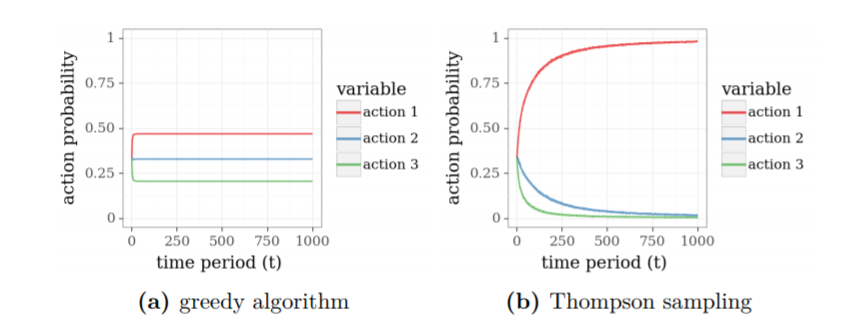
\includegraphics{gandt.png}
\caption{2022-01-14T22\_40\_10}
\end{figure}

    \begin{itemize}
\tightlist
\item
  Second is the UCB algorithm
\item
  The most tricky issue is the Upper Confidence Bound itself. The
  algorithm is too optimistic and gives too much hope to other arms. The
  interval should not enlarge along with the time instead with the grow
  of our confidence we should lay less interest on other arms.
\item
  ​ Another potention issue is that we can not simply use any priror
  information, the confidence interval is determined.
\item
  The last is the Thompson algorithm
\item
  This algorithm is quite fit to this problem. It's based on the
  distribution of Beta, which originally designed to solve problems like
  this. The only con might be we need a quite high-performance beta
  generator at first place and its "robust". We might feel at a lost
  when the bandit is added some extra conditions like cost.
\end{itemize}


    % Add a bibliography block to the postdoc
    
    
    
    \end{document}
